%% This is an example first chapter.  You should put chapter/appendix that you
%% write into a separate file, and add a line \include{yourfilename} to
%% main.tex, where `yourfilename.tex' is the name of the chapter/appendix file.
%% You can process specific files by typing their names in at the 
%% \files=
%% prompt when you run the file main.tex through LaTeX.
\chapter{DressCode}\label{sec:DressCode}

\begin{center}
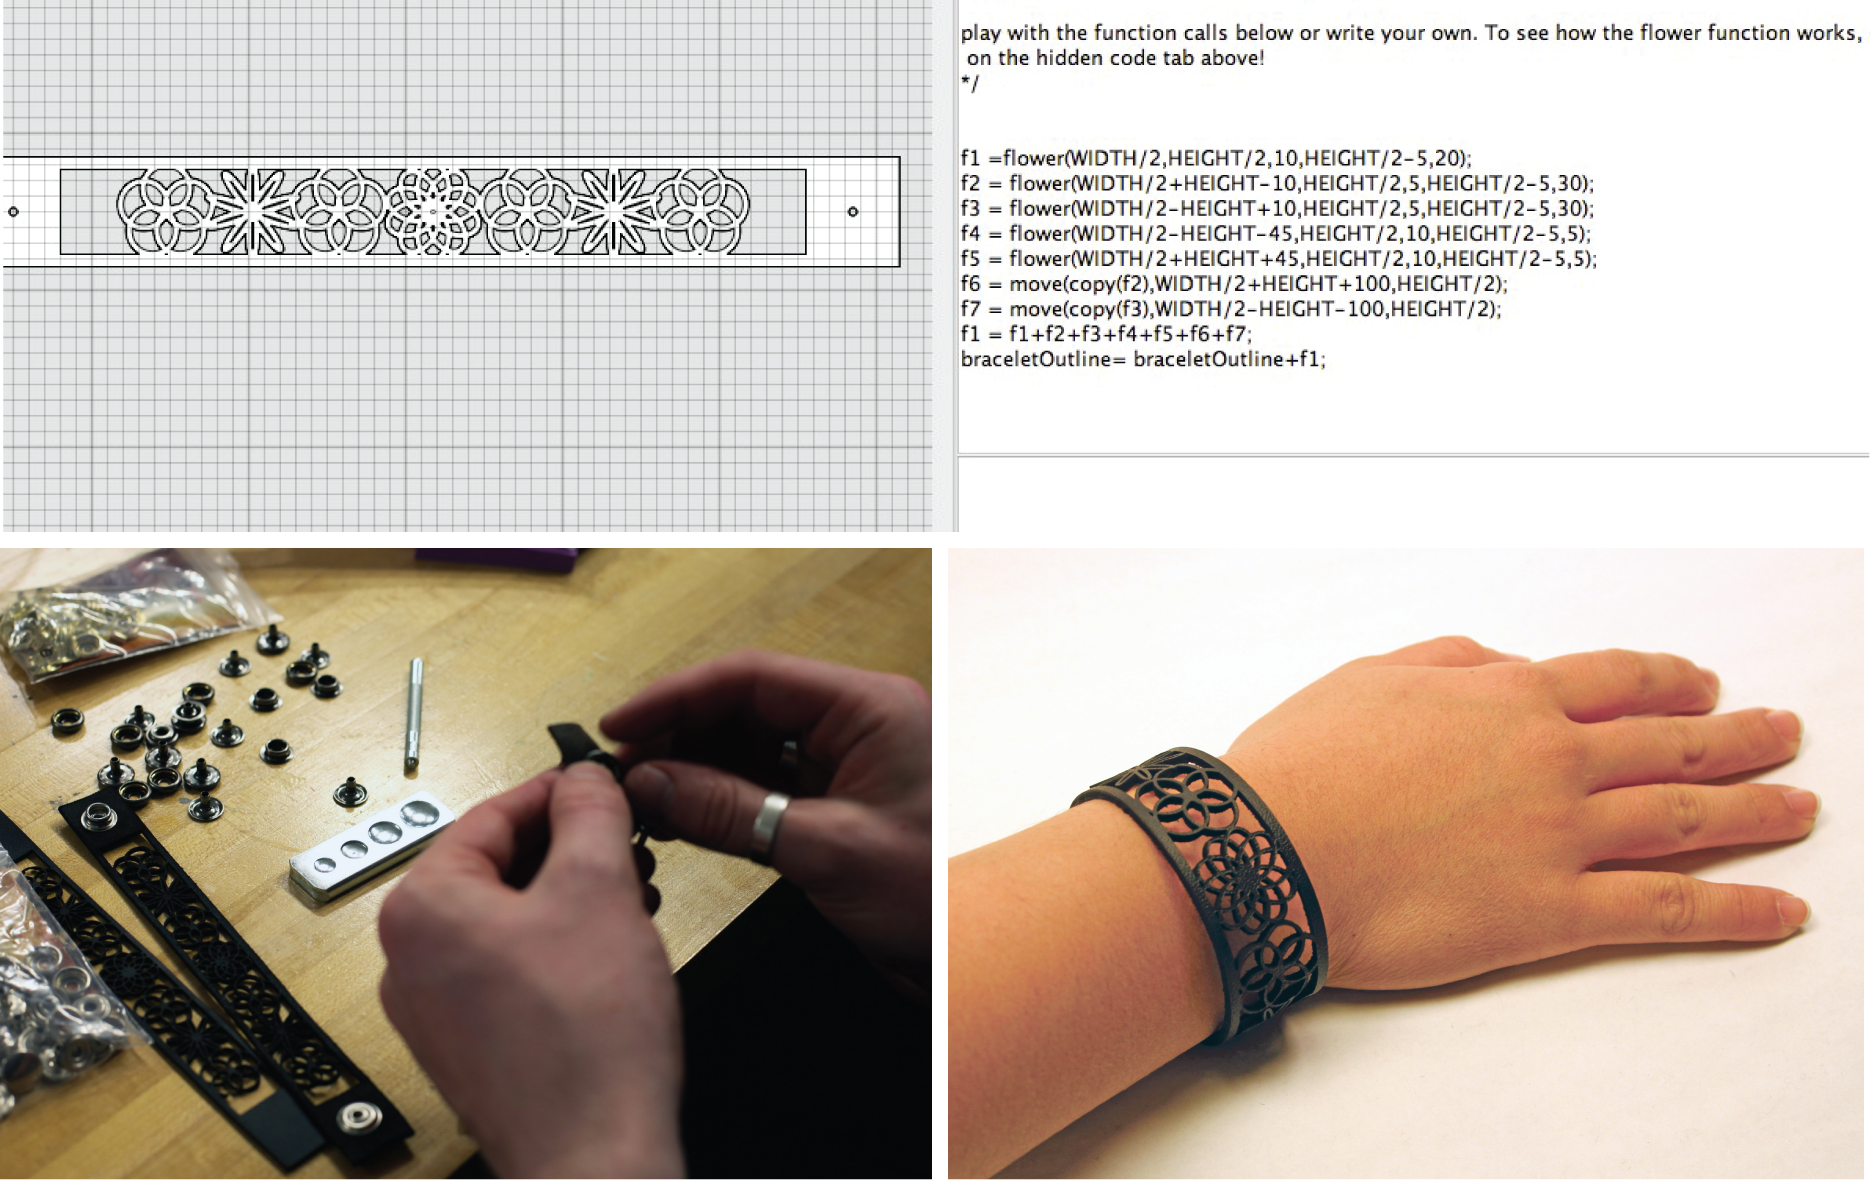
\includegraphics[width=\columnwidth]{images/dressCode_main.png}
\end{center}


The preliminary work of Codeable Objects and Soft Objects clearly demonstrated that algorithmic craft offers a compelling opportunity for personal, creative expression through programming. My goal following these first two tools was to address several of their primary limitations in an effort to better engage novice programers in the computational design aspects of algorithmic craft. DressCode is a stand-alone programming environment and design tool created to support new programmers in open, independent algorithmic craft. To evaluate Dress Code, I conducted two separate day-long workshops, one with experienced programmers and designers, and one for young people who were new to programming. I also worked with FUSE, an out of school STEAM exploration program to develop a set of online activities using DressCode, which are currently in the preliminary stages of evaluation.	 

\section{Design Principles and Software Features}
The focus on fashion in the Soft Objects workshop allowed young people to use computation to create wearable artifacts of their own design. I felt this was a particularly compelling form of engaging young people with computation, and decided to continue working in domain of fashion and garment creation for DressCode. Although the name of the tool reflects an emphasis on fashion, as an application DressCode is general purpose, and can be applied to many forms of algorithmic craft. To preserve the emphasis on fashion, the majority of the example projects and artifacts I  have created with DressCode thus far, are fashion-oriented. The workshops I conducted, as well as the curriculum I helped develop also center on creating wearable artifacts.

With DressCode, I attempted to improve on Soft Objects in several ways. DressCode contains its own programming language with a simplified syntax and a limited set of textual programming methods, to allow people with little or no prior programming experience to work with the language quickly and effectively. The methods within the programming language are developed with digital fabrication applications in mind. They provide the user with the means to design freely, while ensuring that the designs created will translate easily to 2-axis fabrication machines, without the need for additional design software. The DressCode interface is developed to equally prioritize textual programming and visual design, and provide constant visual feedback for programming decisions. The environment has two-panels, one displays a graphic rendering of the user's current design, the other displays their programming code. As a user makes changes to their code, the effects on the design are rendered in the graphic panel. By providing a specialized programming language and immediate support for digital fabrication was to assist non-programmers in independently making design decisions with programming. In short, I wanted to make it as easy as possible for people to decide on their own desired style or aesthetic, and then realize it by writing their own code. The following section describes the features of the DressCode software in greater detail.

\subsection{Interface Design}
 \begin{center}
\begin{figure}[h!]
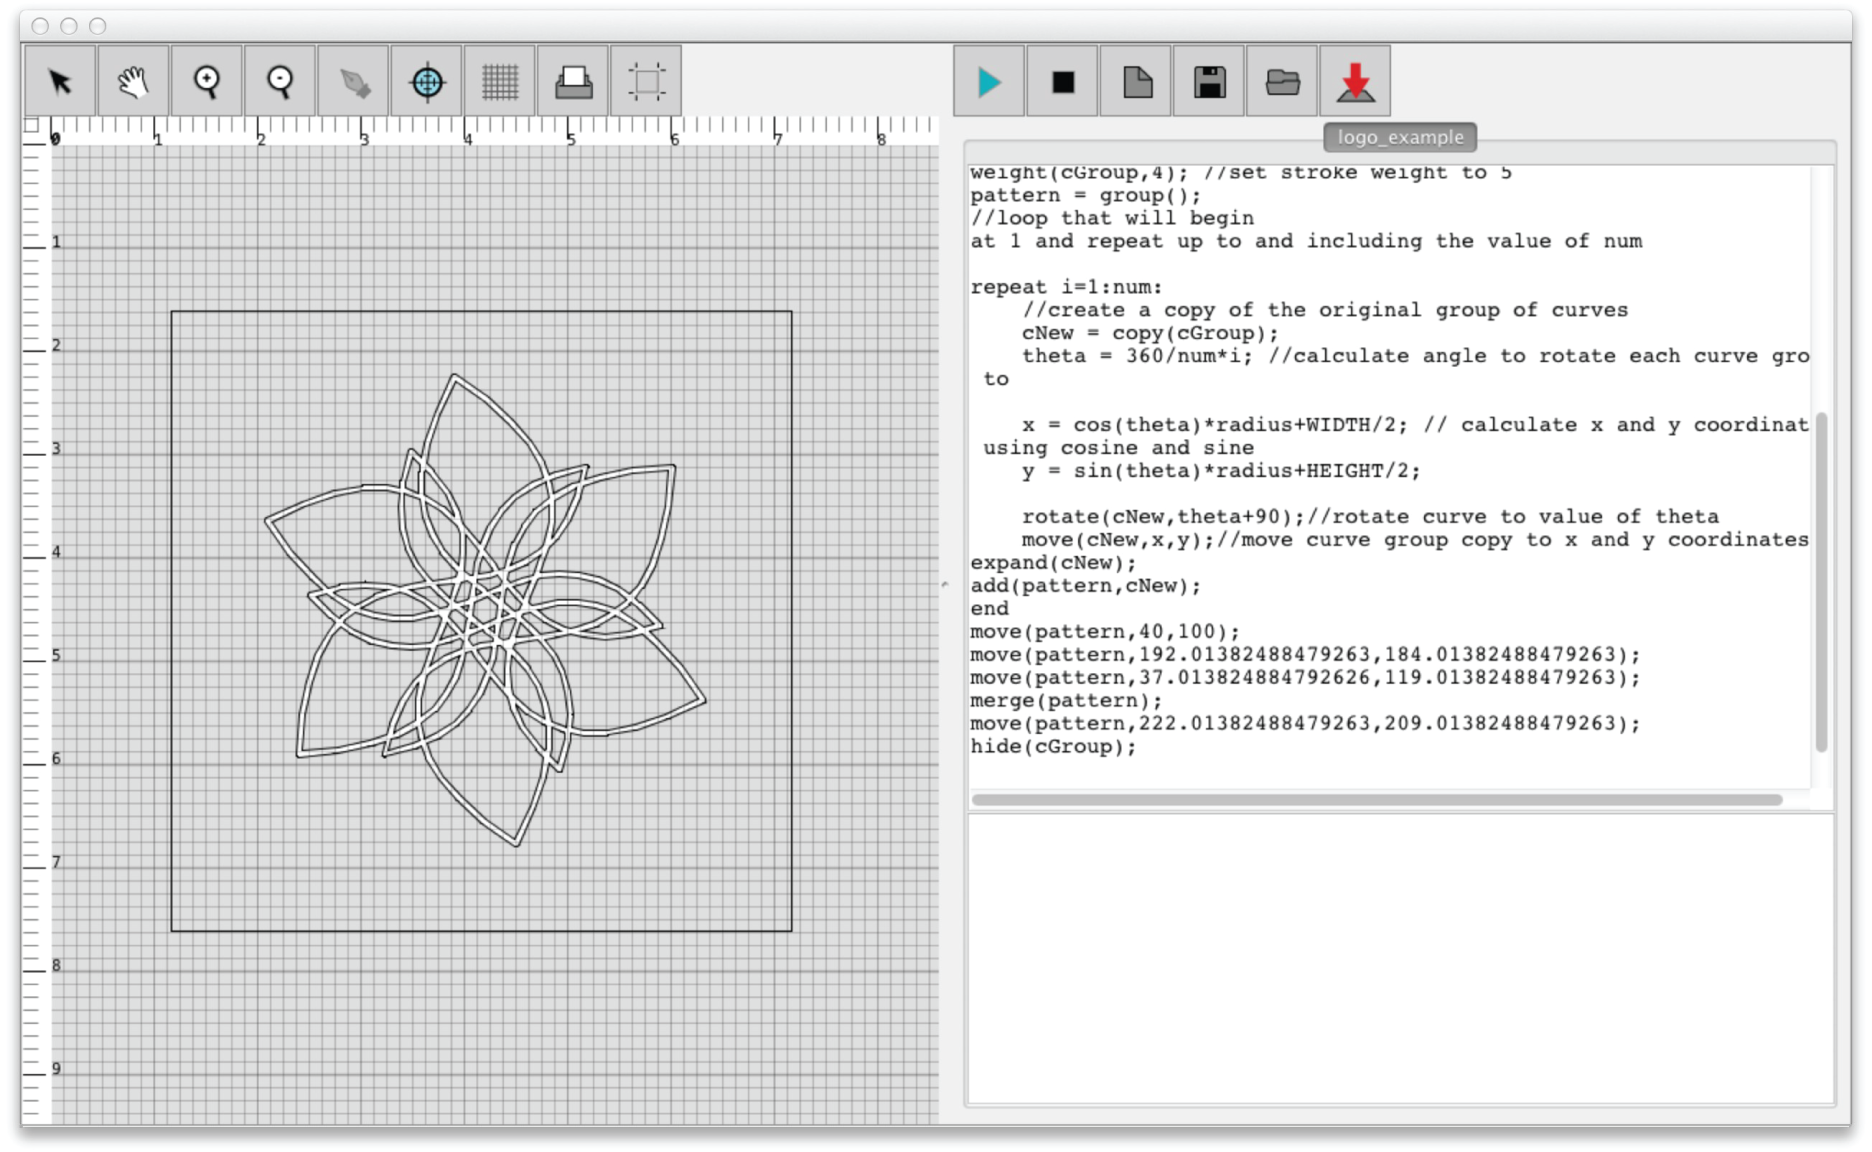
\includegraphics[width=\columnwidth]{images/dress_code_interface.png}
\caption{The DressCode interface}
\label{fig:dress_code_interface}
\end{figure}
\end{center}

The interface of DressCode is divided into two sections, a design panel and a coding panel. The coding panel contains a primary window for entering text, an output console for print output and error reporting. When the play button is pressed, the program in the code window is run and the resulting design is displayed in the design panel. The design panel approximates many of the features of a digital graphic design tool, with rulers and a grid, and a drawing board. The drawing board defines a reference for the coordinate system referenced by the drawing API with the upper left hand corner corresponding to (0,0) in cartesian coordinates. Users can resize the drawing board and set the units to inches or millimeters at any point during the design process. The print button opens a dialog that allows the user to export their current design in a vector format. The design panel also features a set of buttons that allow for graphic manipulation of a user's design. The target button for example, allows the user to graphically select a set of coordinates and have them appear in the programming window as text, and can be used like an eyedropper for pixel coordinates. The plus and minus magnifying glasses and the hand tool are used to pan and zoom in and out of the screen. Lastly, the arrow tool allows for design elements to be graphically selected and manipulated. After a design element is moved with the arrow tool, with the corresponding code for the move appears in the programming window. The graphic components of the the DressCode interface were developed to enable the conceptual and practical execution of digital designs for fabrication, by specifying designs in real-world units. The graphic manipulation tools were designed to be intuitive, while simultaneously working in conjunction with the programming environment, providing people with another method to understand and alter their programs. 

\subsection{Programming Language}
I chose to make DressCode a text-based language because I believe that textual programming languages provide a distinct, and beautiful form of expression that is well suited to design. Textual programming can be considered a form of craft, and in the hands of experienced coders, textual programs can be nuanced, artistic, and finely crafted. I was interested in investigating the ways I could communicate the power and poetic potential of textual languages to people who had never programmed before. With that in mind, I tried to reduce the challenges of first-time programming as much as possible, by augmenting it with graphic interaction and feedback. The DressCode programming language is interpreted with semantic functionality that is simulated through a Java-based library. When a program is run, the design is displayed in the display panel, and any runtime errors are printed to the output console. For most programs, this process is instantaneous, however some programs with complex operations require several seconds to be executed. Interpreting the DressCode language enabled me to greatly reduce the amount of time it took to see changes in a design. I hoped this would provide a greater incentive for people to experiment with their code, and by doing so, allow them to gain a better understanding of how to achieve their personal design objectives.

  \begin{center}
\begin{figure}[h!]
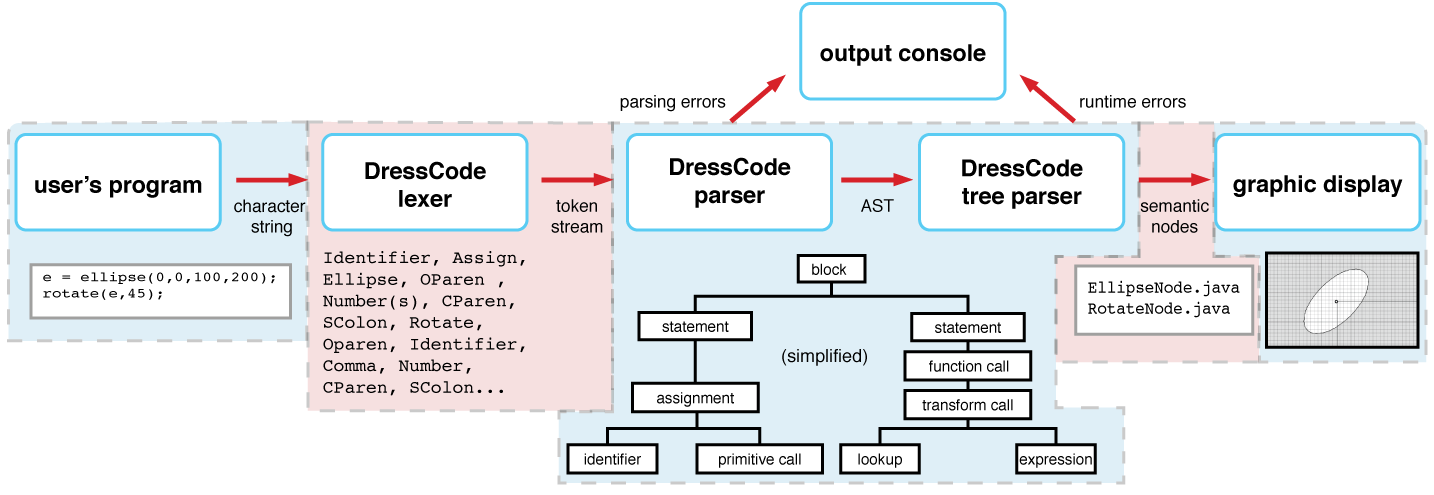
\includegraphics[width=\columnwidth]{images/interpreter_structure_horz.png}
\caption{Interpreter structure}
\label{fig:interpreter_structure}
\end{figure}
\end{center}

 DressCode supports number, string, boolean, and drawable datatypes (figure \ref{fig:basic_datatypes}.) In the Soft Objects workshop, participants often became pre-occupied with memorizing datatypes, and had difficulty knowing which type to declare when creating a variable. To address this barrier, in DressCode, variables are dynamically typed, and can be assigned to datatypes that differ from their original assignment at any point. DressCode determines how to treat the data assigned to the variable based on context. %(figure \ref{fig:variable_assignment}.)

\begin{center}
%\begin{figure}
\begin{lstlisting}
s1 = "hello";
s2 = "world";
s3; //variable without initial assignment

s3 = s1+" "+s2; 
println(s3); //prints hello world

n1 = 2;
n2 = 2.5;
println(n1+n2*10); // returns 27.0
\end{lstlisting}
%\caption{variable assignment.}
%\label{fig:variable_assignment}
%\end{figure}
\end{center}

The  language also contains support for basic expressions, as well as block statements, including conditionals, loops and user-defined functions. Loops are extremely useful for computational design, especially when creating repeating patterns. For new programers however, loops are a difficult concept, and loop syntax is often confusing. I attempted to clarify the loops of DressCode by creating a default update condition, and designating them with keywords I thought would more accurately reflect their function. I also added several methods that allow users to create loop-based patterns with a single statement, by specifying the number of repeats, and the resultant pattern of the loop (wave, arc, grid, spiral or ellipse). 

 \begin{center}
%\begin{figure}
\begin{lstlisting}
//repeat statement
repeat i=0:10:
ellipse(0,i*10,10,10); //draws a vertical row of 10 ellipses
end
\end{lstlisting}
%\caption{loop definitions}
%\label{fig:loops}
%\end{figure}
\end{center}

Custom functions can also be defined by the user, along with any number of dynamically typed arguments. User defined functions are stored in memory and can be defined at any point in a user's program, and called prior to their definition. 
\begin{center}
%\begin{figure}
\begin{lstlisting}
//basic function defintion
def foo(a,b,c):
println(a+b+c);
end

//function call
foo(1,2,3);  //prints 6

//function with return statement
def bar(a,b,c):
return(a*b*c);
end

result = bar(4,5,6)); 
println(result);//prints 120
\end{lstlisting}
%\caption{loop definitions}
%\label{fig:loops}
%\end{figure}
\end{center}

\subsubsection{Drawing API}
 The DressCode API is organized around the creation and transformation of shape primitives including points, lines, curves, polygons, ellipses, rectangles and imported SVG shapes.There is no required "draw" method for DressCode. Instead all primitives are automatically drawn in the display panel in the order of their initialization. This was designed to make it as easy as possible to have one's design appear on the screen. If a user does not want a primitive to appear on the screen, they can hide it.
 
 All primitives can be modified through a set of transformation methods that allow them to be rotated, scaled and moved. Transformations on a primitive are performed by assigning an identifier to the primitive, and then calling the transformation method with the identifier. By using the transformation method to manipulate primitives in a structured manner, it is possible to generate complex and interesting designs from simple forms. Through these methods, DressCode was intended to support the affordances of computational design, specifically precision, visual complexity, generativity and stylistic abstraction, in a way that was feasible for new practitioners.
 
 \begin{center}
\begin{figure}[h!]
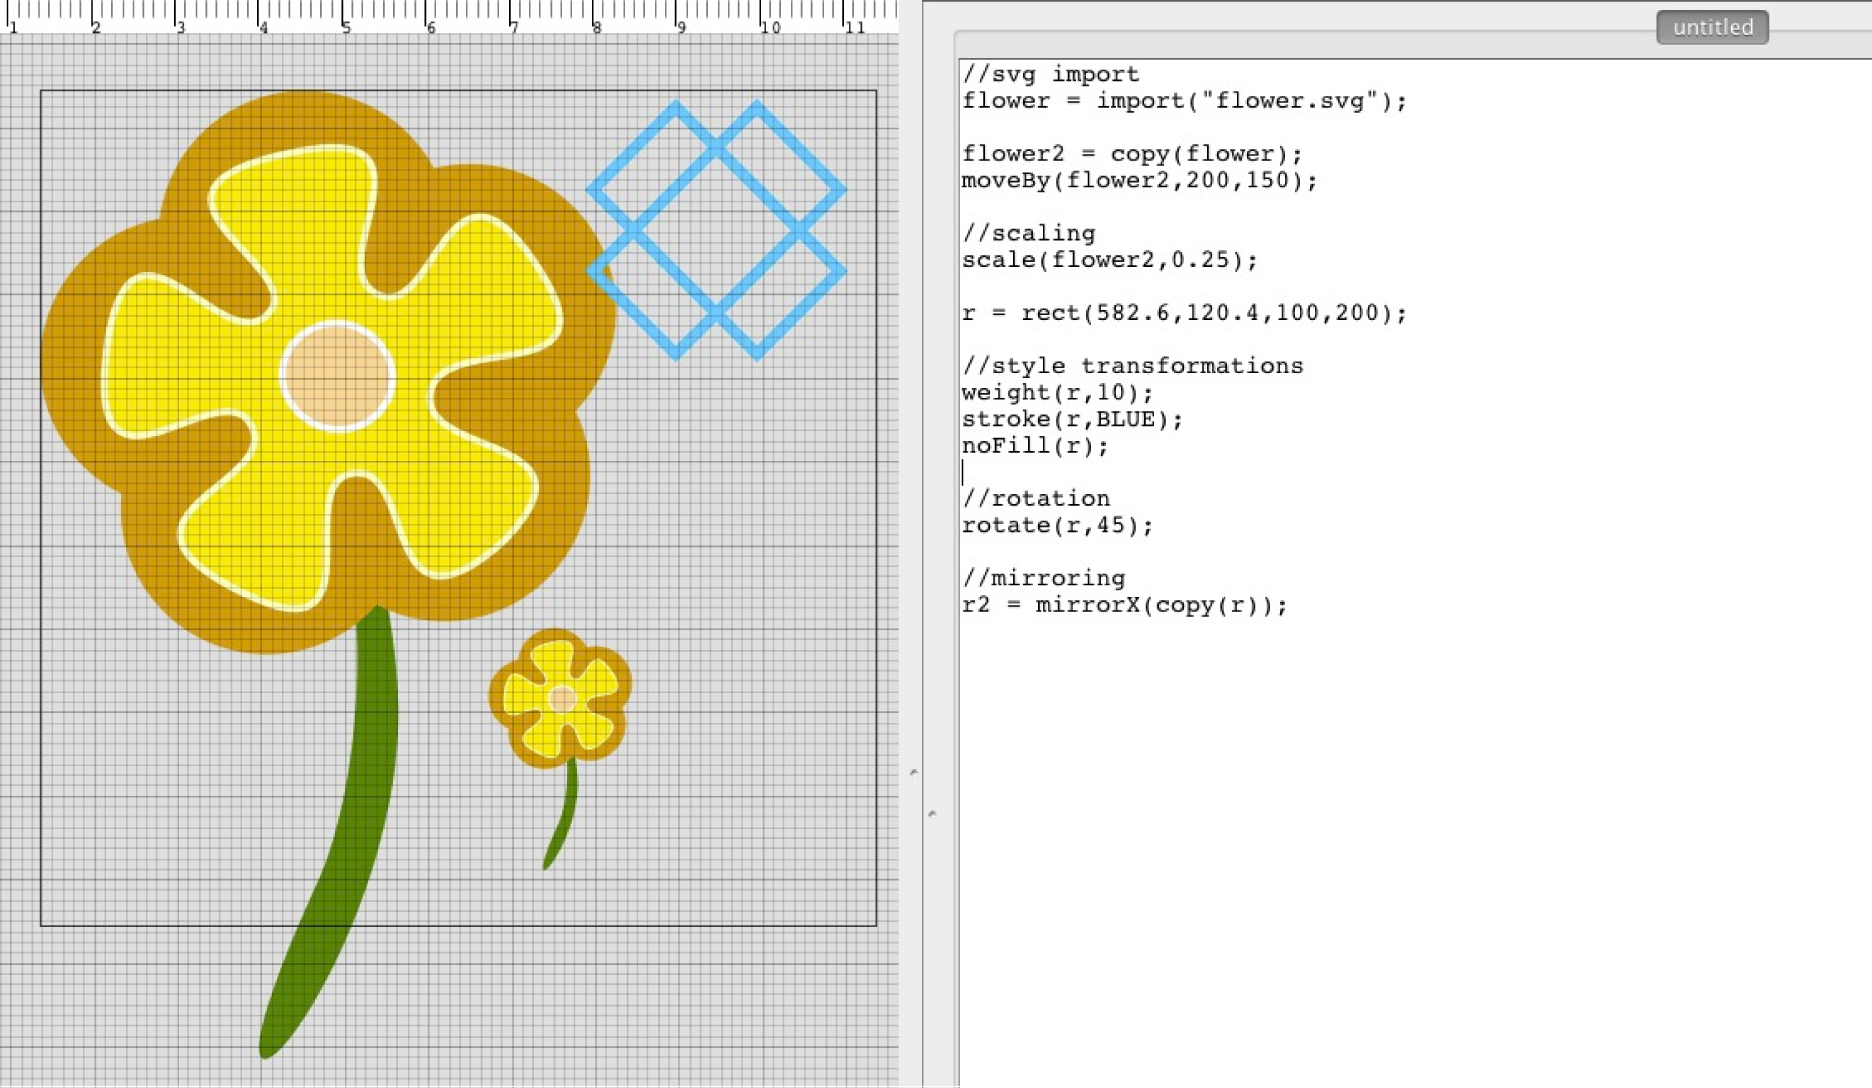
\includegraphics[width=\columnwidth]{images/transformation.png}
\caption{SVG import and sample of transformation methods}
\label{fig:transformation}
\end{figure}
\end{center} 
 
Although I started with a basic set of transformations, I gradually added in additional methods, in response to user testing. This included a moveBy method, a polar move method, mirroring functionality, a copy method, and an addition to the rotate method which allowed a shape to be rotated around a point other than its origin. To encourage generatively, I added a random method, although this raised interesting implementation questions. The random method generates different numbers each time a a program is run, which can be a useful design feature, allowing for the generation of numerous patterns with random variations. Figure \ref{fig:random_symmetry} demonstrates variations of an algorithm that produces randomly symmetrical stripe patterns.  It can also be potentially problematic, when the user wishes to keep the same randomly generated number for each interpretation of their design. 

 \begin{center}
\begin{figure}[h!]
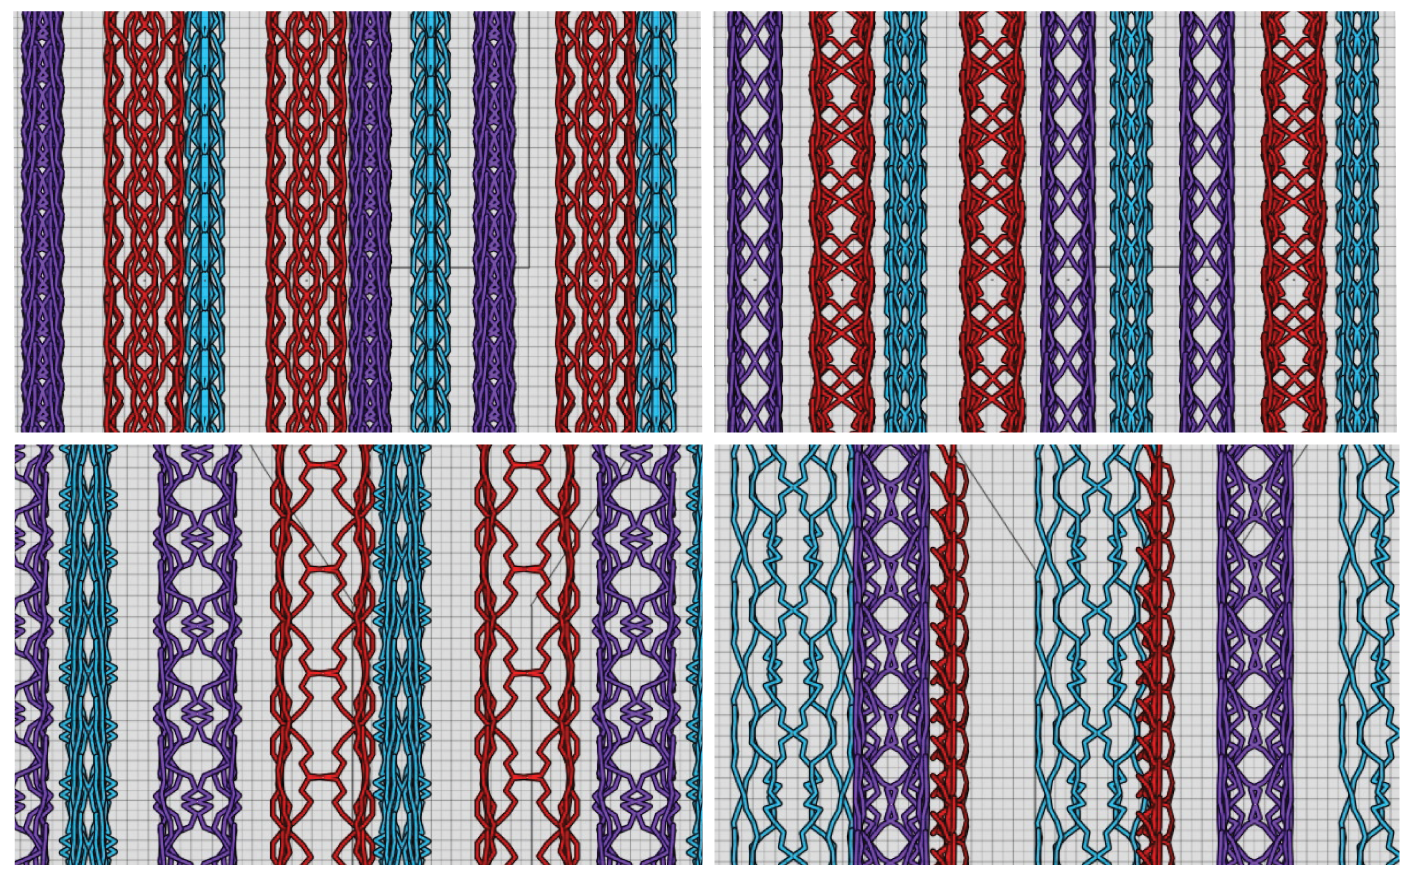
\includegraphics[width=\columnwidth]{images/random_symmetry.png}
\caption{Stripe pattern variations using the DressCode random method }
\label{fig:random_symmetry}
\end{figure}
\end{center}

\subsubsection{Polygon Booleans:}
Polygon boolean operations are techniques that allow shape primitives to be combined and subtracted from one another in various ways. Polygon booleans are widely used in CAD applications and are essential for many forms of digital fabrication because they allow for complex configurations of shapes to be combined into effective toolpaths. Polygon Boolean operations are also important from a design perspective, because they facilitate the creation of new forms, not possible through other drawing techniques. Processing does not contain methods for polygon booleans. As a result, in the Soft Objects workshop we had to rely on Adobe Illustrator to prepare designs for fabrication, which was confusing, disruptive to the design process, and time consuming for the participants.  Therefore, it was important to me that DressCode contained native polygon boolean operations which better supported digital fabrication, and  were conducive to the design process. DressCode contains methods for performing unions, intersections, differences and either-or intersections between any two or more shapes. These methods enable users to combine objects and create complex polygons with multiple holes. operation. They can also clip shapes within clipping masks based on the dimensions of the design they are creating. They can also expand strokes to filled polygon paths, enabling the translation of line art to a form that will maintain its appearance when fabricated. By positioning these operations as primary components of the DressCode, I attempted to create a programming language that produced forms that were applicable to fabrication as a direct result of the design process, rather than requiring an extraneous post-processing step that could interfere with the aesthetics of the piece. In this way, users could be in control of their design throughout the entire process of programming, fabricating and crafting. 

 \begin{center}
\begin{figure}[h!]
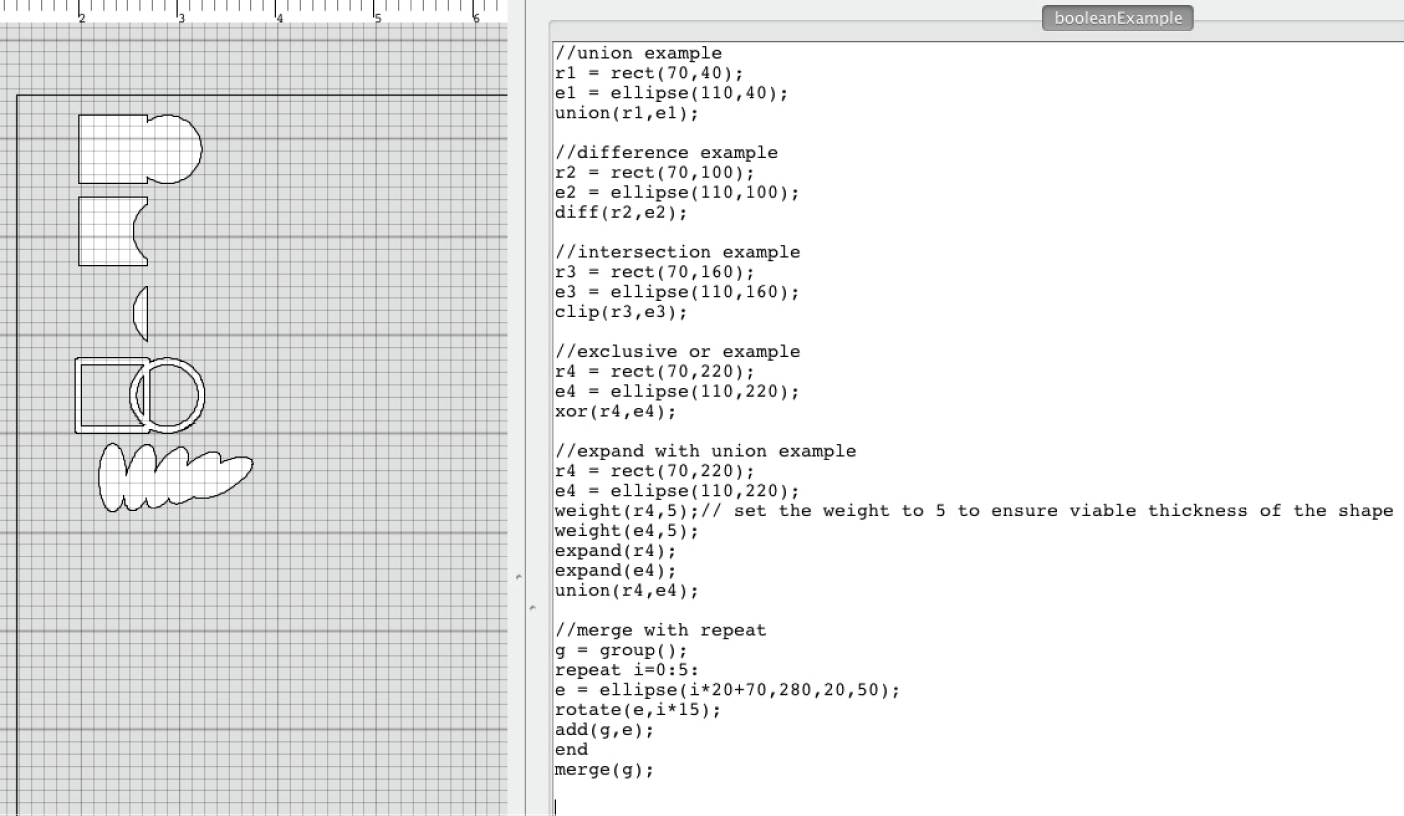
\includegraphics[width=\columnwidth]{images/boolean.png}
\caption{Polygon boolean operations}
\label{fig:boolean}
\end{figure}
\end{center} 

\subsubsection{Grouping}
One major concern in computational design is how to effectively organize and collectively manipulate complex designs with many individual elements. To address this, DressCode primitives can also be programmatically grouped, allowing for transformations to simultaneously be applied to multiple elements. Groups have their own origin, which is used as the reference point for all move, rotation and scale methods applied to the group (figure: \ref{fig:grouping}.) The groups in DressCode provide structural mechanism that bridges computational data structures with organizational structures found in non-computational graphics software. Groups are treated similarly to lists in that they can be populated through a loop, and individual objects can be accessed and manipulated by via their index. Similar to Adobe Illustrator and many 3D modeling programs, groups can also be moved with the graphic manipulation tools, and have boolean operations performed on all of the members simultaneously. This connection creates a more balanced treatment between properties of digital graphics software and computational affordances, to better communicate the utility of lists in a design context. Groups also provide a practical advantage for digital fabrication, as they can be automatically merged upon export, returning a single complete tool path that conducive to subtractive fabrication processes.

 \begin{center}
\begin{figure}[h!]
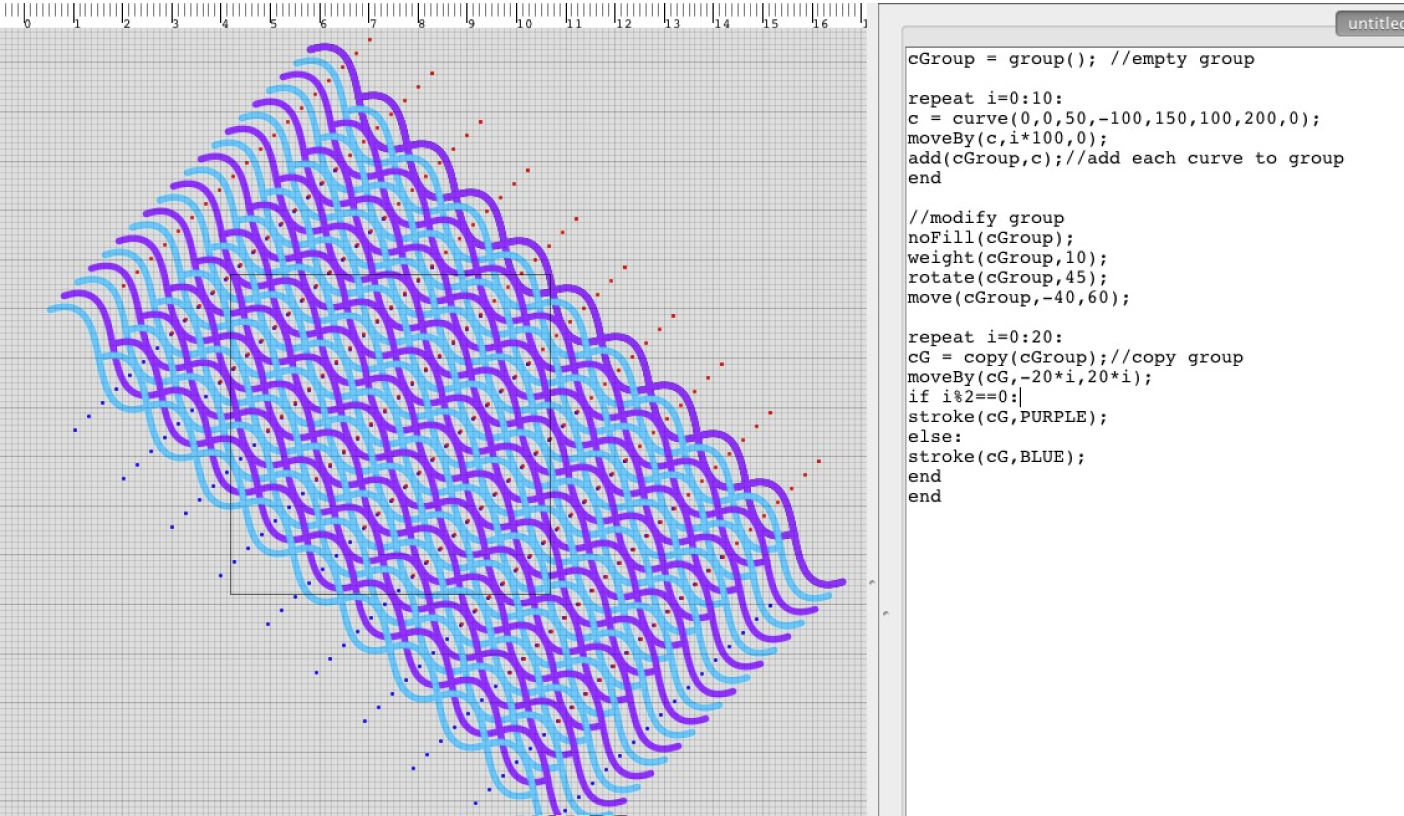
\includegraphics[width=\columnwidth]{images/grouping.png}
\caption{Grouping with transformation and repeat statements}
\label{fig:grouping}
\end{figure}
\end{center} 

\subsubsection{Informational Methods}
Computational designers do more than specify designs. They also must be able to access information about components of their design, and make aesthetic or practical decisions based on that information. DressCode features a set of methods that return information about shape primitives, such as their location, origin point, width and height, as well as a method to determine the Euclidean distance between two objects. I also added a set of methods that allow the conversion of pixel values to inches, centimeters and millimeters, or in the current units of the drawing board. These methods encourage designers to evaluate their designs on practical and aesthetic criteria, and allow them to ensure their creations fit the correct parameters for physical construction. 

\section{Fabrication and Crafting Processes}
Because DressCode is intended for algorithmic craft, it had to enable people to translate the designs created in the software to functional physical artifacts. DressCode can export vector files that can be used with any 2-axis fabrication machine. Depending on the materials and machines available, a wide variety of end products are possible. A large component of developing DressCode involved experimenting with different fabrication machines, crafting techniques and end artifacts. I tested the resultant pieces from these fabrication processes with different crafting techniques that ranged in difficulty. Highly accessible techniques included making artifacts that required basic paper-folding or iron on appliqu�s for clothing. More difficult techniques included sewing garments, screen printing onto fabric, and jewelry making. 

Because accessibility was a primary goal, it was important to ensure that DressCode could be used with widely available forms of digital fabrication. I experimented with the laser cutter and CNC milling machines with DressCode however I  also developed a set of projects that were compatible with the cameo craft vinyl cutters, and standard inkjet printers. These options lowered the cost for participation in algorithmic craft for many individuals and groups. I also used DressCode in conjunction with two on-demand online fabrication services,  Shapeways and Spoonflower, to produce 3D-printed jewelry and larger inkjet printed garments. 

The support of algorithmic craft depends on more than good software. It is also important to convey information about material affordances for different forms of fabrication, instructions for combining craft construction methods with fabricated pieces, and inspiration for possible projects and end artifacts. The study of methods for documenting and communicating this information is substantial, and could easily constitute its own thesis. For DressCode, I attempted to experiment with fabrication techniques and projects that were interesting to me, and that I believed would be accessible and compelling for young people.  To provide support for independent users, my undergraduate research assistants and I created a set of example templates in DressCode that are directed towards specific end projects and fabrication machines (figure: \ref{fig:dresscode_examples}). We also began documenting some of the crafting techniques required to complete these projects online. I also worked with FUSE, an interest driven STEM exploration program in Chicago, to document DressCode. With FUSE, I developed an online activity designed to help young people use DressCode to create vinyl cut accessories \footnote{https://www.fusestudio.net/challenge/dresscode/shrink-it}. Despite these initial explorations, there still remains significant research to conduct in the process of documenting and conveying fabrication and craft knowledge in conjunction with computational tools.
 \begin{center}
\begin{figure}[h!]
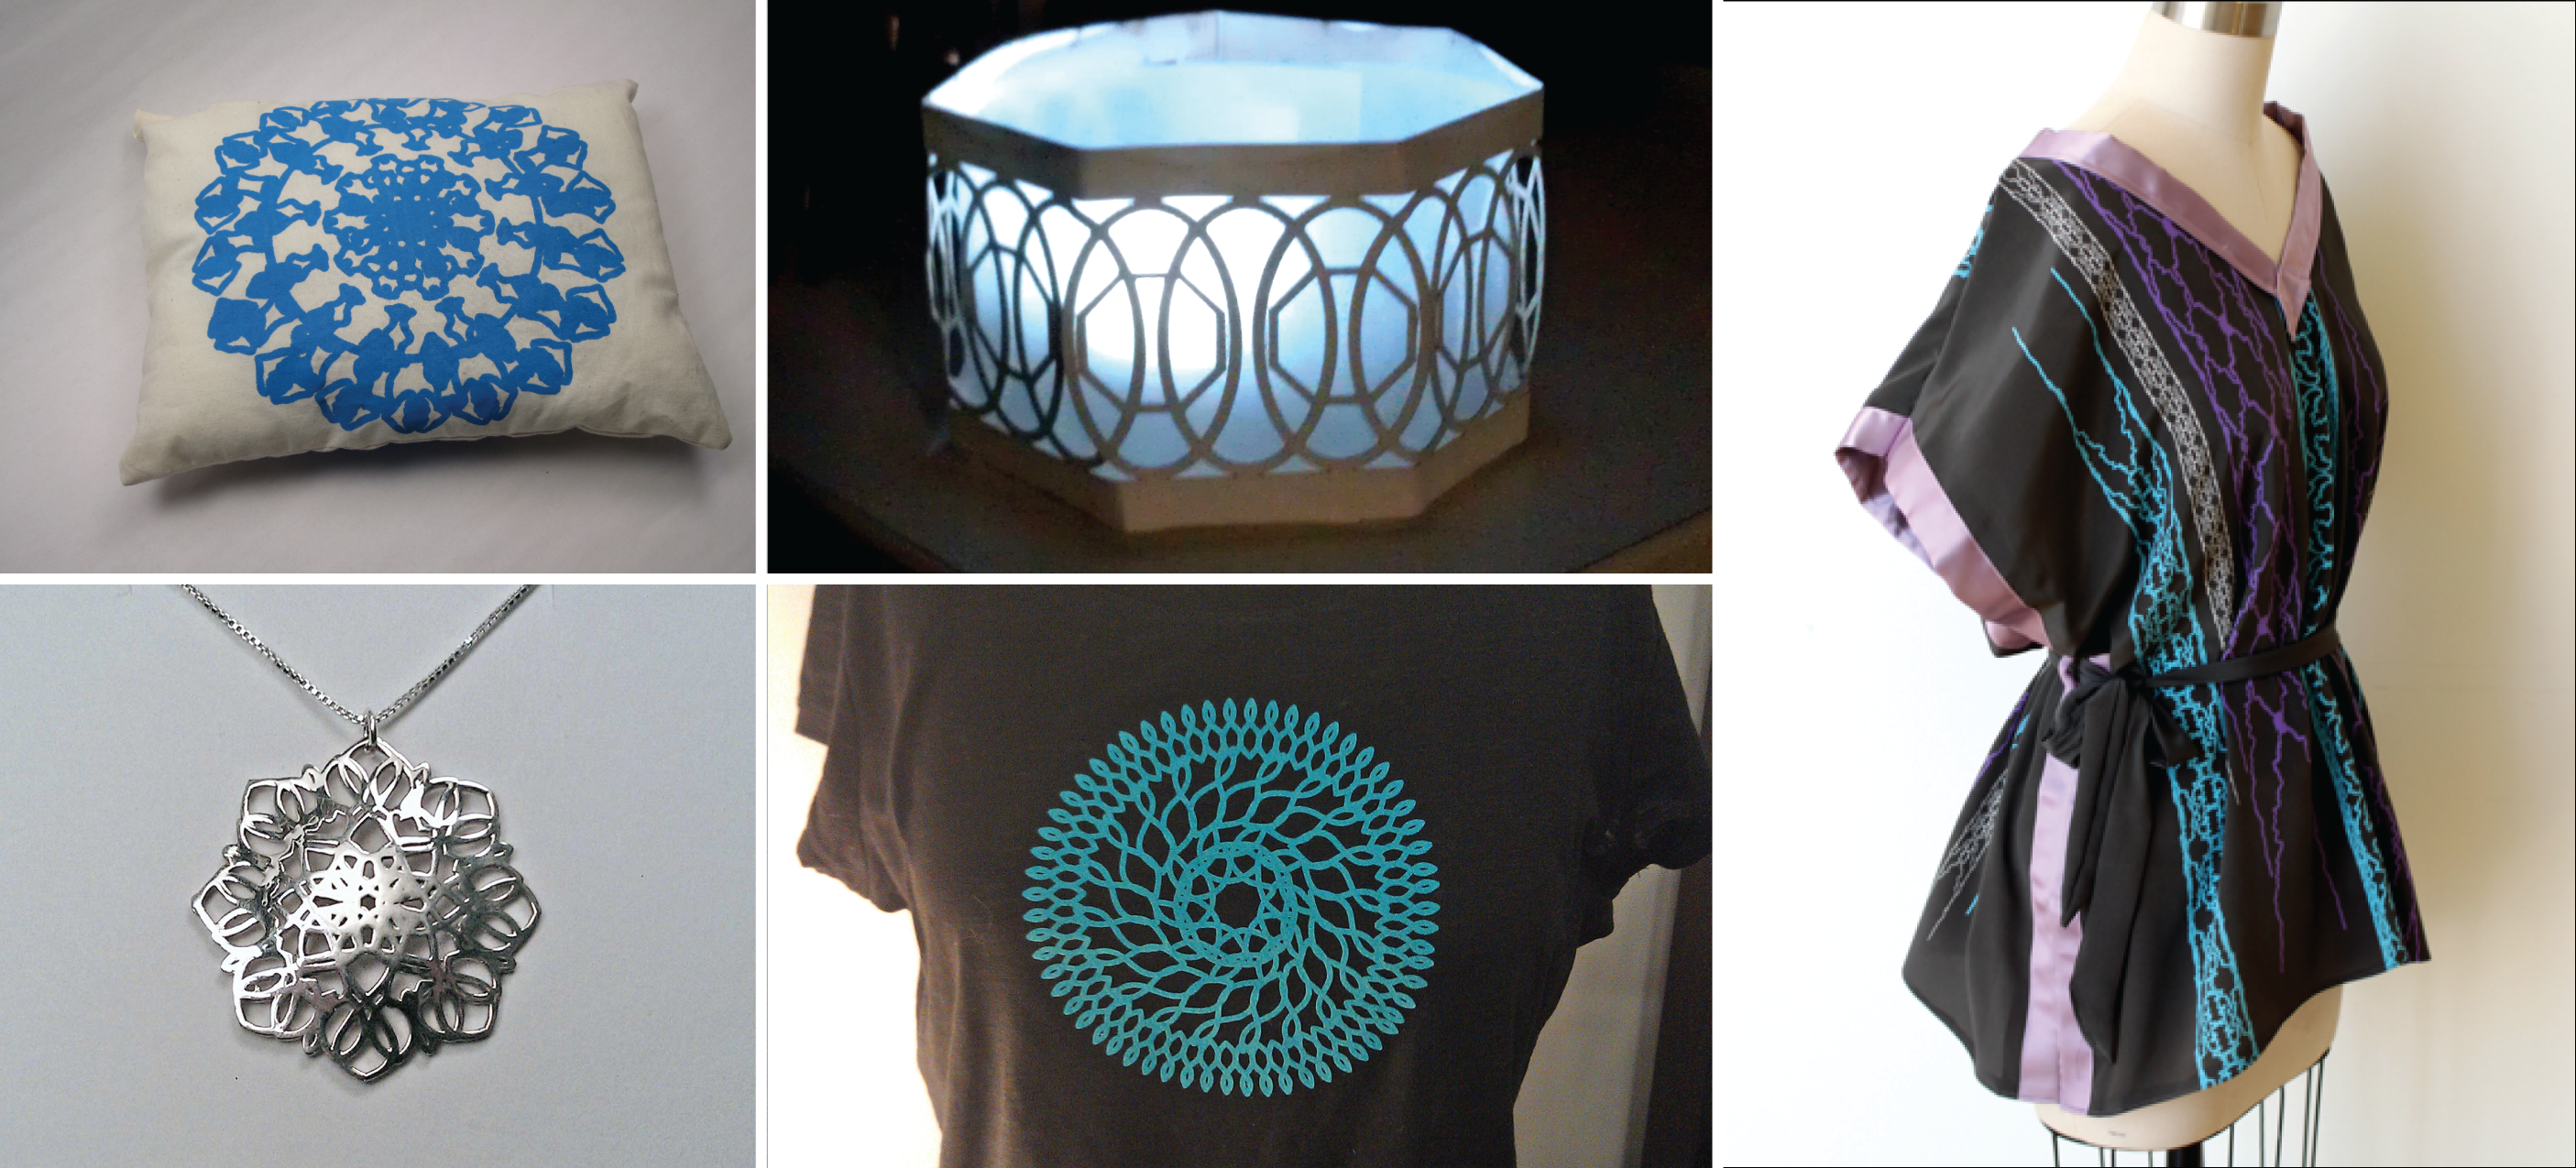
\includegraphics[width=\columnwidth]{images/dresscode_examples.png}
\caption{Several example artifacts created with DressCode Designs (clockwise from top left: vinyl-cut screen printed pillow, vinyl-cut tea light, ink-jet printed silk caftan, laser-cut iron-on tshirt, 3d printed silver pendant) }
\label{fig:dresscode_examples}
\end{figure}
\end{center}

\section{Tool Summary}
The DressCode programming language, graphical interface and craft and fabrication documentation materials are designed to work in combination to extend the creative opportunities of algorithmic craft while reducing the technical difficulties of using programming to design for digital fabrication. The drawing methods are created to be easy to use, but broad in their creative possibilites. The interface mixes programming functionality with rapid visual feedback and graphic manipulation. The documentation and curricula provide assistance in using digital fabrication machines, and ideas for possible end projects, helping people to translate their designs to functioning crafts. By allowing people to produce complex structures from simple forms, and realize these forms in personal physical artifacts, my intention is to instill confidence in people's ability to program, while generating excitement and enjoyment of the the creative opportunities inherent in algorithmic craft.


\section{Workshops}
To evaluate the success of DressCode in helping young people participate in algorithmic craft, I conducted several user studies and workshops. I informally tested DressCode with members of the FUSE development team, and with the staff at Dream Yard, an after school STEM education space in the Bronx. Following these tests and a period of additional development, DressCode was evaluated during two separate day-long workshops at the MIT Media lab. The first workshop was conducted among experienced designers, artists and programmers, who were selected individually from MIT, Harvard and the Cambridge community. The second workshop was conducted among ten young adults selected from youth organizations in Cambridge and arts-and-craft workshop mailing-lists at MIT. Participants in both workshops used DressCode to create laser-cut leather crafts. By testing DressCode with experts and young people, I hoped to learn about its usability for the target demographic, and also gain insight into future directions and design techniques to incorporate into the tool. 

\subsection{Expert Workshop}
The expert workshop was comprised of eight participants between the ages of  19 to 33. Five of the eight participants were female, and all had prior experience in programming. 75\% of the participants indicated a strong prior interest in design, and 50\% enjoyed crafting. All participants had formal training at a college level in either art, design or computer science. 

The expert workshop was structured as an open-ended design activity. I began the workshop with a 30 minute discussion on the connections and intersections between design, arts and crafts and programming. Following this discussion the, participants were given a 45 minute tutorial on the basics of the DressCode, after which participants were given access to the online code reference and a physical handout with quick references for some of the key methods. I also provided participants with a leather bracelet template and several example programs that generated different patterns for the template. Participants were given the option to design within the template, but were also free to create whatever they wanted.  After participants spent several hours designing, they were shown the basic fabrication process, and provided with materials consisting of several varieties and colors of leather. Participants then had 3-4 hours to finish the design of  their piece. As they completed their designs, they were taken in groups to the shop to fabricate their parts and then given access to craft tools and a variety of fasteners (snaps, rivets and jewelry connectors) to convert them into finished artifacts.

\begin{center}
\begin{figure}[h!]
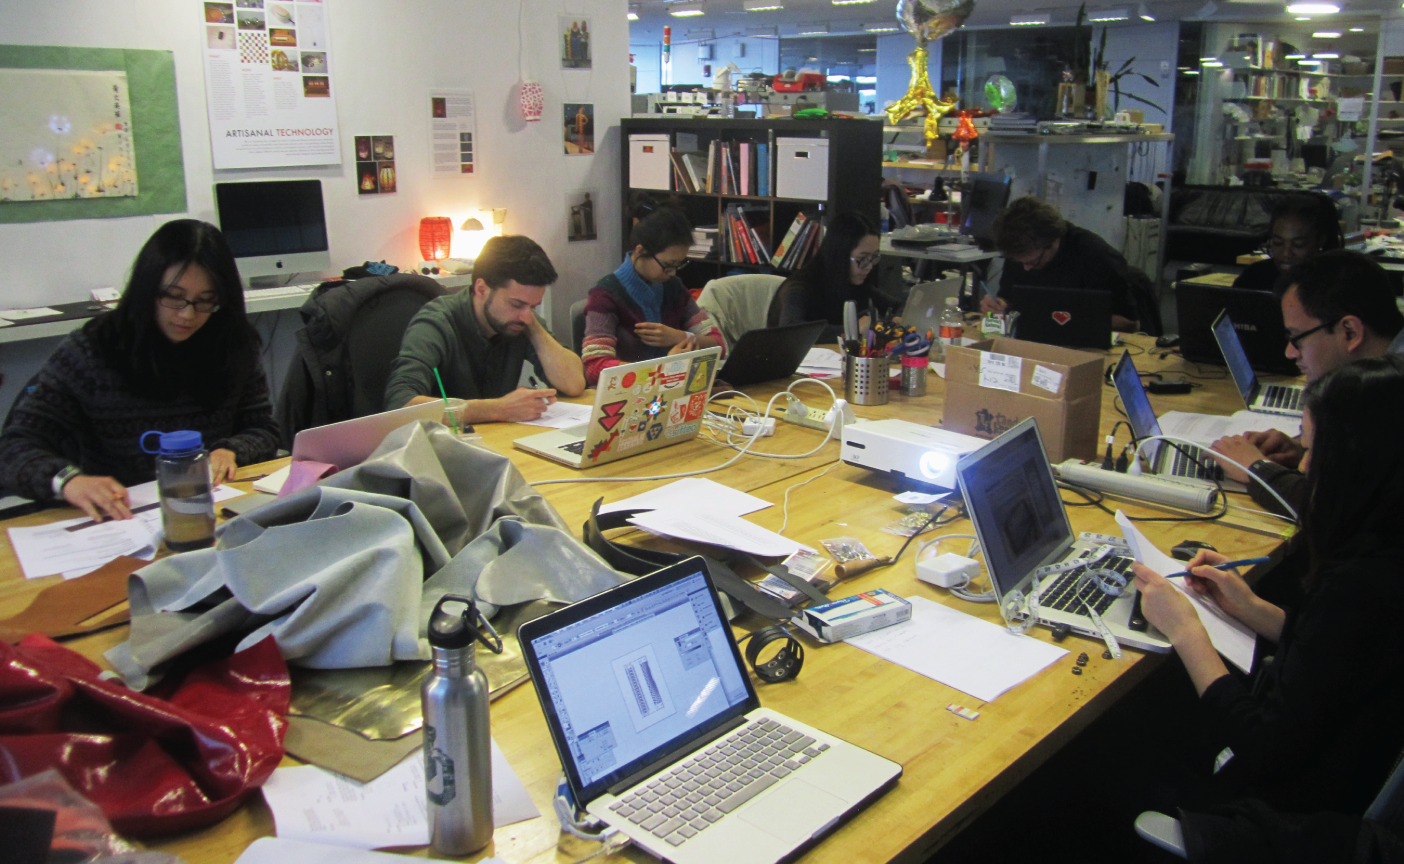
\includegraphics[width=\columnwidth]{images/adult_design_time.png}
\caption{The expert workshop}
\label{fig:adult_design_time}
\end{figure}
\end{center}

\subsection{Youth Workshop}
The youth workshop was conducted among ten young adults, aged 15-17, 20\% male and 80\% female. Five of the youth participants were participants in the Teach 2 Learn, Learn 2 Teach program in Boston \footnote{http://learn2teach.pbworks.com}. Of those surveyed, three participants had prior experience with Scratch, and two had worked with the Arduino programming environment in a prior Media Lab workshop.  All of the participants said they had some prior experience in art, design, or craft.  Prior to the workshop, 60\% of the participants indicated that they did not feel comfortable programming on their own, however the majority indicated that they were interested in learning more about the process. 

The youth workshop was more structured than the expert workshop with the goal of helping to familiarize participants with the possibilities and affordances of computational design and fabrication. During the workshop, I was assisted by two Media Lab students and an undergraduate research assistant.  We began by passing out three colors of post-its for the categories of of art and craft, design and programming. We then held a 5 minute brainstorm where we asked each participant to write down people, tools, ideas and projects the associated each category on the respective colored post-it. After, we collected the post its, and put them up on a board in related clusters, and used the resulting associations to instigate 30 minute discussion on the participants ideas about the connections between the three domains.  We ended the discussion by talking about some of the possible craft applications of computational design, and began the introduction to DressCode.

\begin{center}
\begin{figure}[h!]
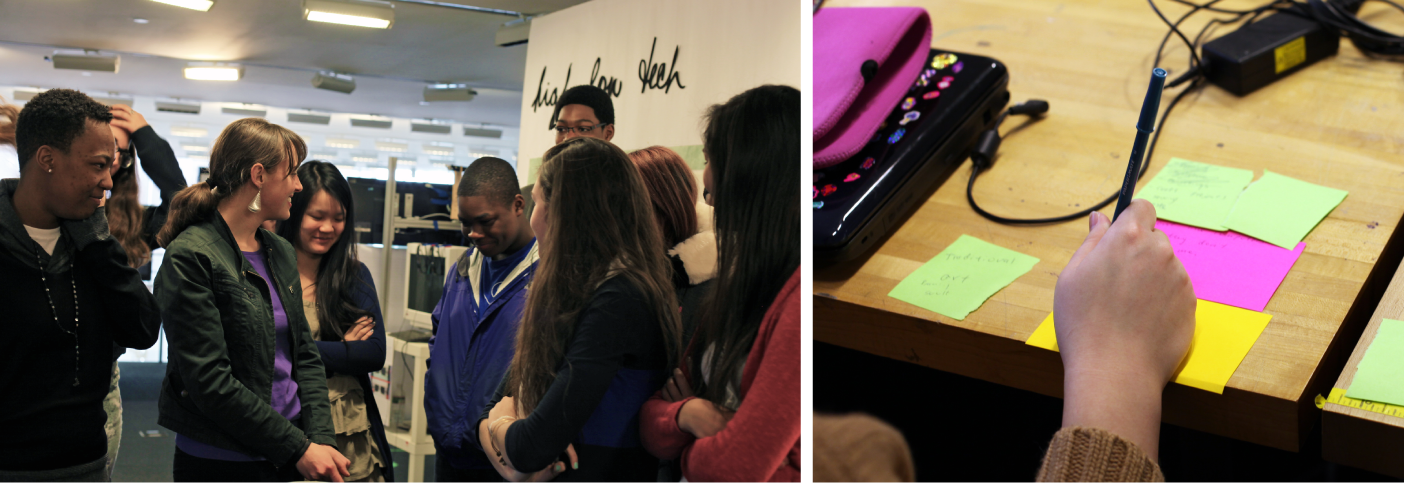
\includegraphics[width=\columnwidth]{images/youth_brainstorm.png}
\caption{The youth brainstorm and discussion}
\label{fig:youth_brainstorm}
\end{figure}
\end{center}

All of the design work in the youth workshop was structured around the concept of radial symmetry. Radial symmetry provides a good introduction to algorithmic craft because it is a relatively easy pattern express mathematically, and serves as an excellent motivation for using a loop. Radial symmetric patterns are commonly found in nature, making it possible to use radial orderings of shapes to generate designs that are biological in appearance. In addition, radially symmetric forms are often aesthetically appealing to people.  To introduce the youth to computational design, I explained the concept of DressCode and then spent 20 minutes leading the group, step by step through the process of creating a basic algorithm that created a radially-symmetric form(figure: \ref{fig:starting_algorithm}.) After every participant had successfully created their version of the algorithm, I showed them how they could use the same algorithm to create different designs by changing the number of iterations of the loop, the type of shape that was drawn, and the width and height of the shape. Participants then had 15 minutes to experiment with different parameters, and produce different designs, followed by a group show and tell session (figure: \ref{fig:show_and_tell}.) 

\begin{center}
\begin{figure}[h!]
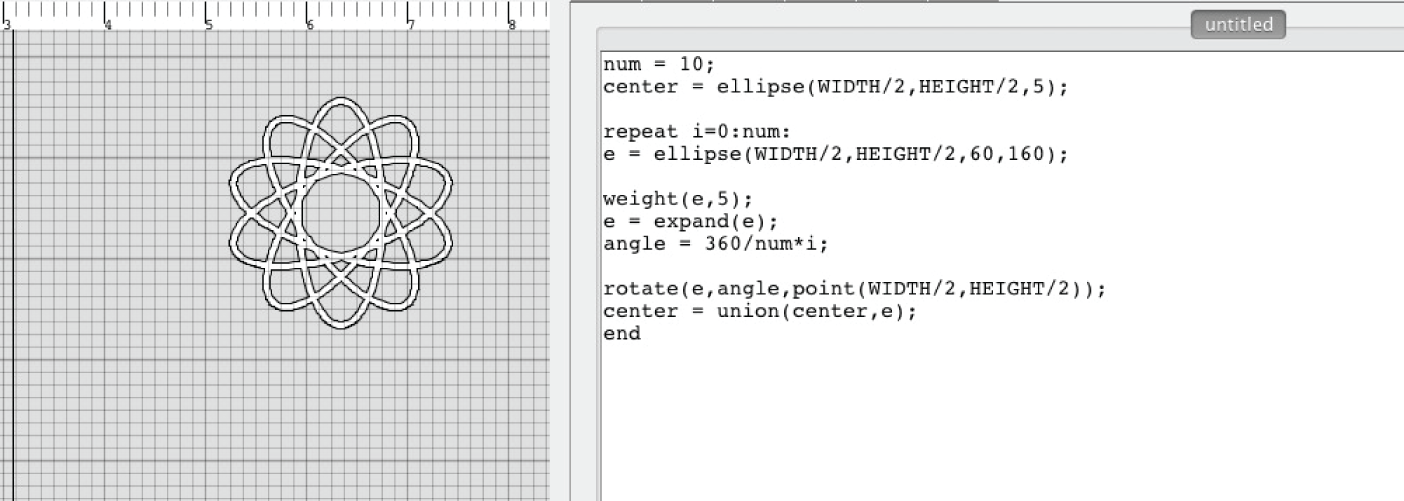
\includegraphics[width=\columnwidth]{images/first_algorithm.png}
\caption{The first algorithm learned by the youth participants}
\label{fig:starting_algorithm}
\end{figure}
\end{center}

\begin{center}
\begin{figure}[h!]
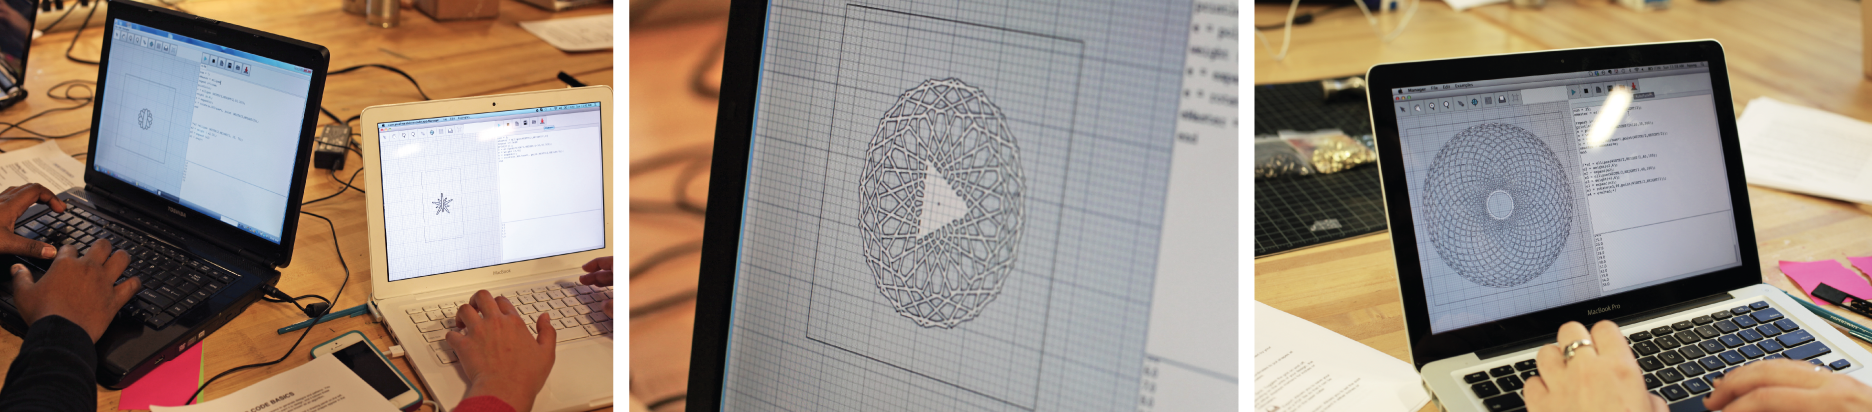
\includegraphics[width=\columnwidth]{images/show_and_tell.png}
\caption{Some example variations on the first activity}
\label{fig:show_and_tell}
\end{figure}
\end{center}

Next, the participants were provided with example programs that contained a bracelet template. The example programs featured a pre-written function that duplicated the algorithm they had written in the previous activity, with arguments corresponding to same values they were manipulating before. Participants were then given time to use the function to make multiple elements of the original radial pattern with different parameters. A second tab in the example program revealed the code for the radial function, which they could modify if they desired. The example template was constrained so that the dimensions of the bracelet would automatically correspond to the size of the drawing board. By measuring their wrist and resizing the drawing board, they could generate a bracelet of the correct size, and maintain their original design (figure: \ref{fig:bracelet_template}.)

\begin{center}
\begin{figure}[h!]
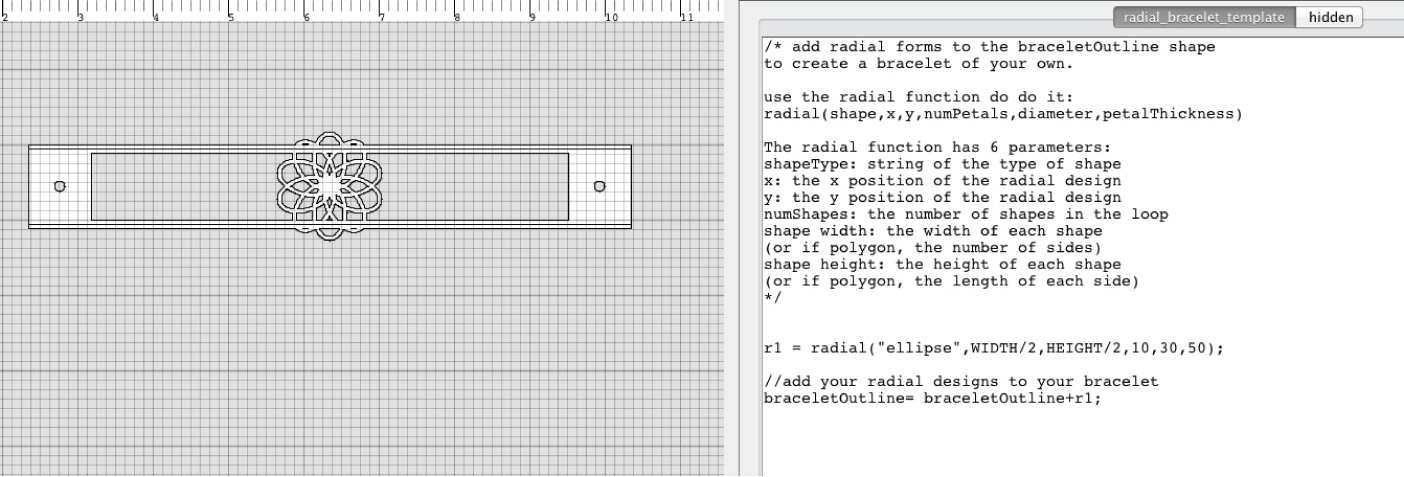
\includegraphics[width=\columnwidth]{images/bracelet_template.png}
\caption{The bracelet template with one instance of the radial function being called}
\label{fig:bracelet_template}
\end{figure}
\end{center}

Participants were given two hours of free design time. When they had settled on a final design, they first printed out a paper copy and ensured that it fit their wrist. Following that, they selected their material and were taken in groups to the laser cutter. Afterwards, they were shown how to attach the fasteners to the bracelet, and provided with tools that allowed them to alter their piece by hand. 

\section{Results}
\subsection{Expert Results}
All but one participant in the expert workshop indicated that they were able to successfully able to complete a finished product. The types of end products varied.  While many participants produced leather cuffs, people also created finger puppets, earrings and a belt using the software. There was a high degree of variation in the algorithms used to create the finished products. Several participants relied exclusively on the radial symmetry algorithm, but others created patterns with computationally ordered curves, rectangles and lines in different arrangements.  The participant who created the leather belt designed the pattern so that it demonstrated the evolution of the algorithm that comprised it; as the individual patterns progress across the length of the belt, they grow in complexity. 

Because of the high degree in variation among approaches and end products, conducting the expert workshop was difficult. Many of the participants began with design goals that were at odds with the affordances of DressCode, such as creating representational characters in the case of the finger puppet example.  In addition, several of the end projects required instructor intervention to ensure they were suitable for fabrication, because of their complexity. Overall, the expert workshop produced a promising set of physical artifacts and demonstrated the limitations and benefits of using DressCode across a broad range of design approaches. The expert participants also provided feedback on specific features to incorporate into future versions of the DressCode software. The random method and unit conversion methods were added directly following the workshop based on participant suggestion.

\begin{center}
\begin{figure}[h!]
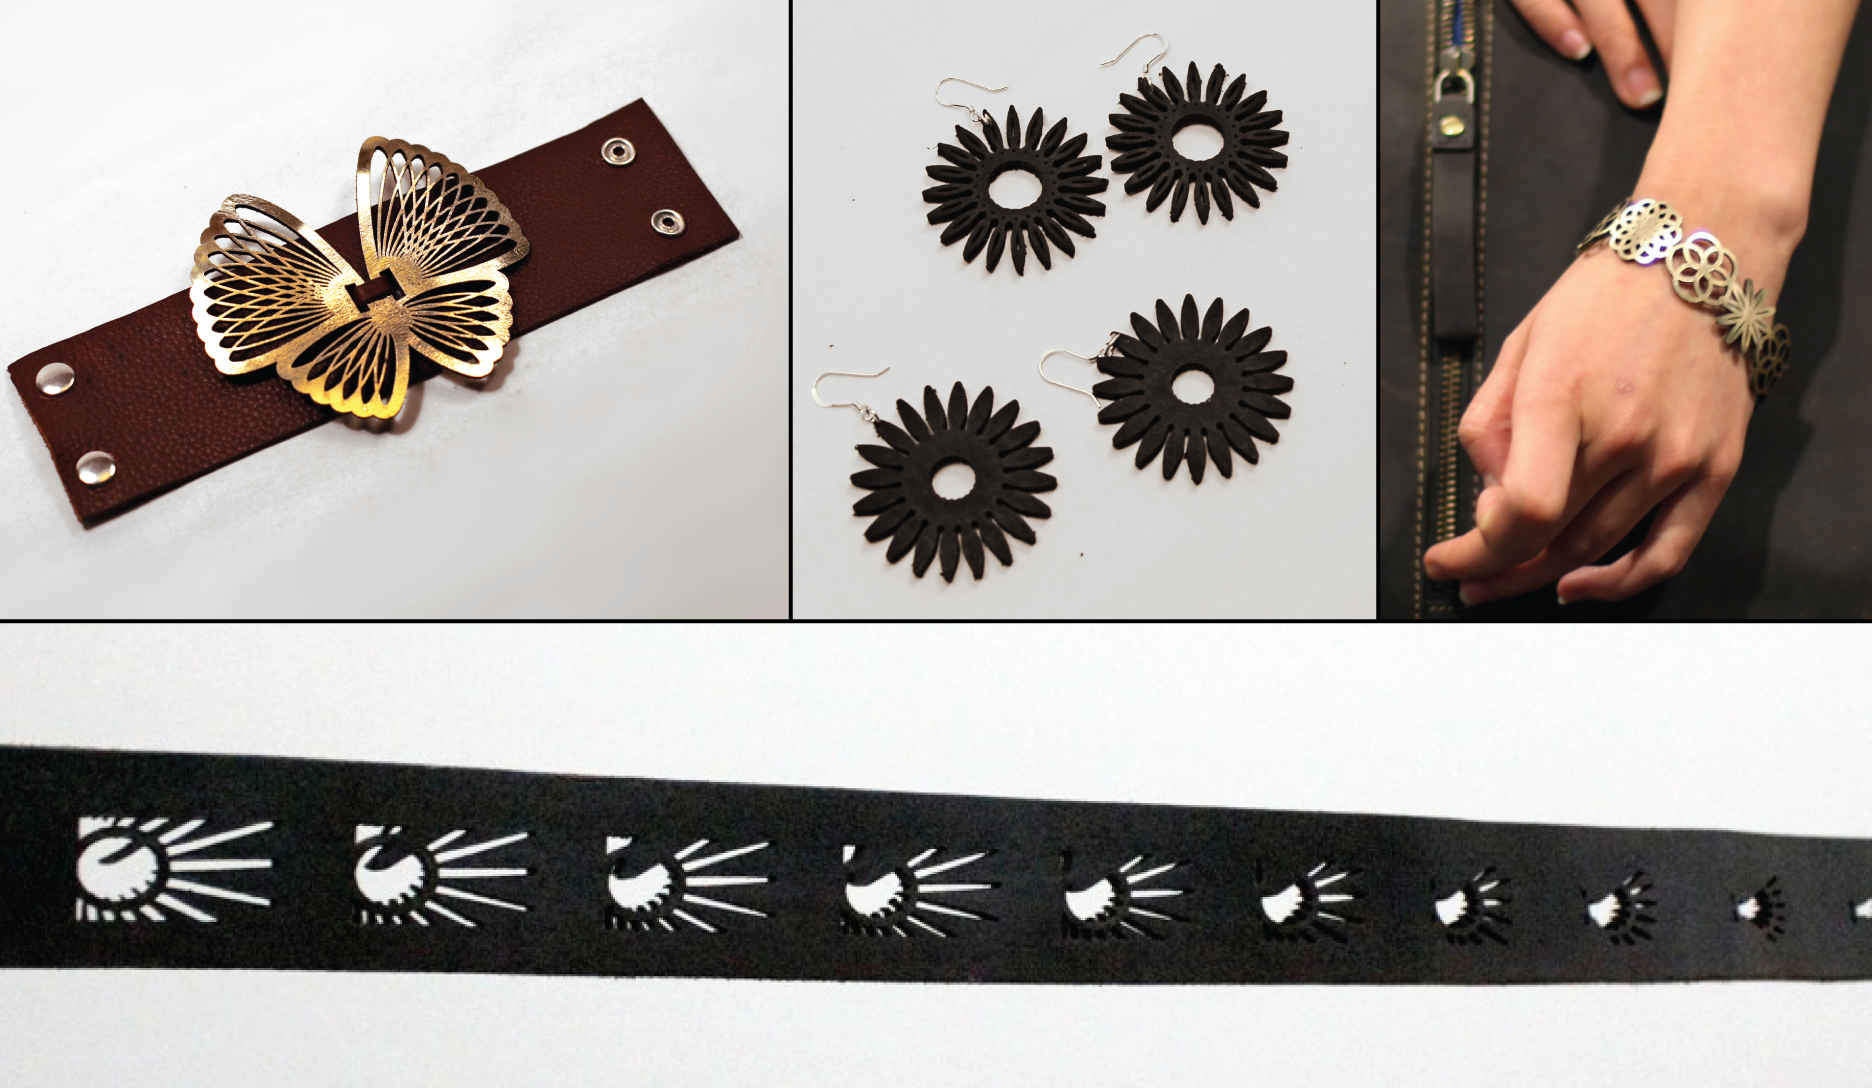
\includegraphics[width=\columnwidth]{images/expert_results.png}
\caption{a sample of the completed projects from the expert workshop (clockwise from top left: butterfly cuff, leather earrings, patent leather bracelet, algorithmic progression belt)}
\label{fig:expert_results}
\end{figure}
\end{center}

\subsection{Youth Results}
Because the youth workshop was more structured than the expert workshop, the participants in it produced a more consistent set of physical products. All participants in the youth workshop were successfully able to use DressCode to produce a unique leather cuff (figure: \ref{fig:youth_results}.) Even though every person made the same type of artifact, the patterns and approaches among the bracelets were very different. Some were geometric, some were floral, and some of the styles were difficult to link back to the original radial algorithm. Each participant was also able to successfully write their own radial symmetry algorithm in the initial lesson and produce a variety of patterns with it, which many translated to their bracelets. During the bracelet design portion, several participants directly modified the algorithm in the template to better fit their design goals, and went beyond the bounds of the original program. Eight of the participants  said they planned to wear the bracelets they created during the workshop, however two indicated that they planned to give them as gifts, rather than keep them for themselves. A comparison of the pre-and post-workshop surveys showed that several of the participants' comfort in programming increased following the activity. After the workshop, more participants indicated that they thought programming was a good tool for personal expression and design. All participants stated that they believed they could use programming to make things that were beautiful, whereas several had disagreed with this statement before the workshop.

\begin{center}
\begin{figure}[h!]
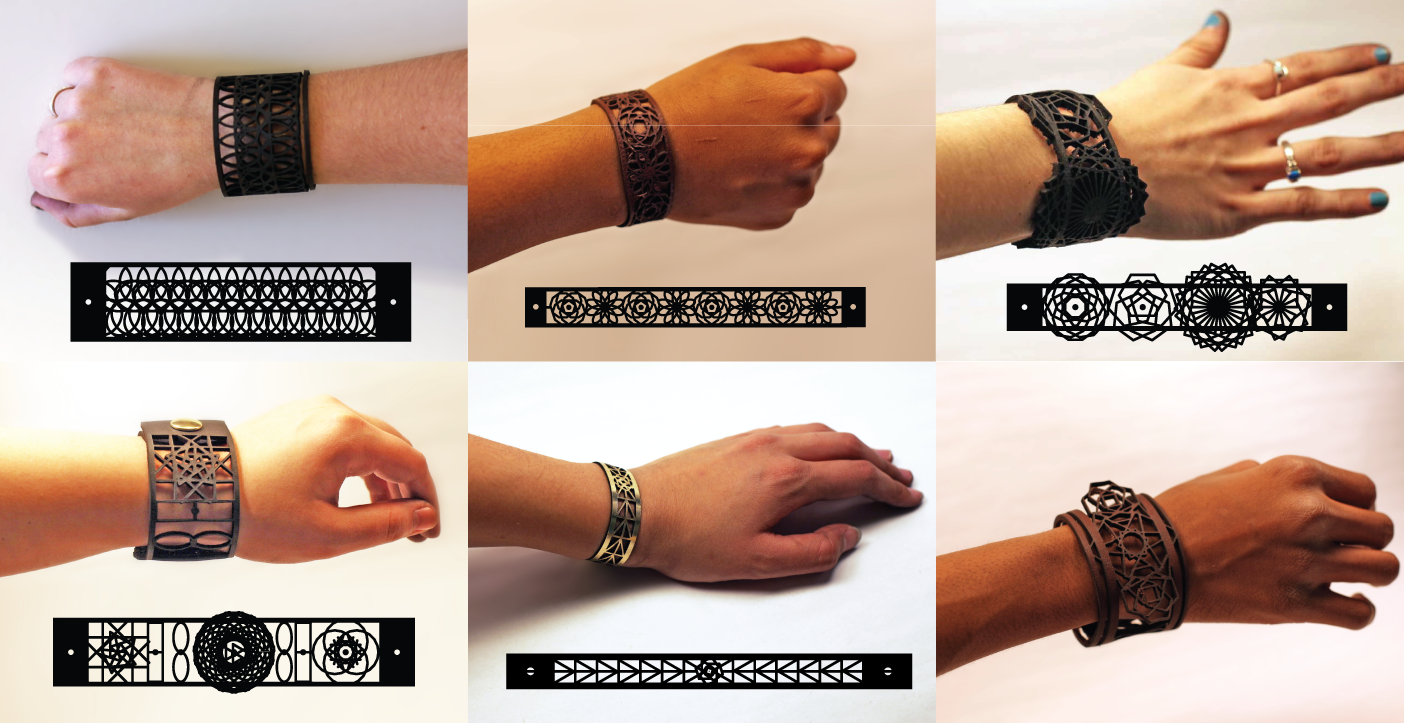
\includegraphics[width=\columnwidth]{images/youth_results.png}
\caption{a sample of the completed leather cuffs from the youth workshop}
\label{fig:youth_results}
\end{figure}
\end{center}
%\section{Curriculum description}
%\section{Preliminary curriculum results}
\section{Discussion}
The DressCode workshops re-affirmed many of the benefits of algorithmic craft  that were apparent through Soft Objects and Codeable Objects. Through DressCode people were able to express their personal aesthetic preferences by working with computation, digital fabrication and craft. Participants also demonstrated new confidence and and independence in programming and design, and a greater awareness of the applications of computation. The experience was enjoyable, but also intellectually challenging, leading to strong sense of  accomplishment among participants. 

The DressCode workshops also revealed new aspects of algorithmic craft, not apparent in earlier studies.  Young people were discovered to have strong prior associations about programming and craft that were counterproductive to preparing them for the challenges of building objects by hand. In addition, although computational aesthetics are often abstract, in the hands of young designers, they can convey personal symbols, narratives, and signifiers of gender that are extremely powerful when realized in a wearable artifact. Lastly, algorithmic craft artifacts are ascribed a special value by young people that blends the affordances of craft and computation; the artifacts are special because of the programming code that produces them, and their one-of-a-kind rarity as an object.

\subsection{Starting Notions of Craft and Computation}
When developing a tool for combining craft and computation, it is important to understand people's prior conceptions in these areas. In the case of the DressCode study, there was a strong distinction between the views of the two groups of participants on the respective roles of craft and computation. During the expert discussion, two separate forms of craft were discussed. People acknowledged that craft could be viewed as hobby and amateur practice, however they also demonstrated an appreciation for craft as an artisinal practice. In artisanal crafts, artifacts held higher value than mass produced ones because of the time and expertise required for their production. In the youth discussion, the appreciation of artisianal craft was completely absent. Instead the young participants considered all forms of craft as accessible recreational activities. This distinction was surprising. Although the perception of craft as open and accessible has its benefits, many youth participants dismissed the difficulty of craft in comparison to programming. One young woman articulated her view on the difference between writing a program and throwing pottery, stating that she knew she could throw a pot, but that she would be unable to write a program, despite having no prior experience in either medium:

\begin{quotation}
\textit{``It's just a whole new program, it's not something that I already know how to do. Arts and crafts is like, anybody can do it, but here you need to follow what [the instructor] says, you need to know what you're doing ... I think you just need to have more forehand knowledge to know what to do."}
\\Youth Participant S.M.
\end{quotation}

There was also a difference between the amount of variation in the crafting processes between the two experts and young people. Several participants in the expert group experimented with layering different materials on top of one another for a different effect. One participant sewed a portion of her project rather than attach portions with snaps. Another used the snaps as an aesthetic component, by placing them across the length of the piece and then snapping on different colored pieces of leather in different patterns. There was limited variation in the approaches the youth practitioners took in the crafting portion. Most stopped after they had attached snaps to their bracelets. The youth participants consistently described the craft component as difficult, and even stressful at times:
\begin{quotation}
\textit{``Something that was difficult was hammering the snaps in straight enough for them to function well."}
\\Youth Participant F
\end{quotation}
\begin{quotation}
\textit{``It was enjoyable being able to wear it and making sure that it would fit. It was a little stressful figuring out how to put the clasp on. "}
\\Youth Participant K
\end{quotation}
\begin{quotation}
\textit{``I think the actual physical copy [of my bracelet] is slightly less attractive than the one I had on the computer."}
\\Youth Participant C
\end{quotation}
\begin{quotation}
\textit{``I hate being anxious because I don't know if it's going to come out right. I like the designing on the computer, but once it comes out it looks like crap. So I'm really happy that I came to this (workshop), this is the first one that came out."}
\\Youth Participant ST
\end{quotation}

The frustrations experienced by youth participants in the craft stages of their projects correspond to similar frustrations from participants in the Soft Objects and Codeable Objects workshops. The discussions with the participants on their conceptions of programming and craft at the start of the workshop now provide more context for the cause of this frustration. It is likely that people become frustrated during the hand construction components not merely because craft is difficult, but because they have prior conceptions of craft as accessible, and expect to be successful at it upon their first attempt. Conversely, participants in the workshops are often convinced of their inability to program, so any degree of success represents a significant accomplishment. One of the challenges in engaging people in computation is in convincing them that programming is not as hard as they think. When engaging young people in craft, this challenge is reversed; people should be encouraged to consider craft as a broad field with the potential for difficulty. Successfully aligning and hammering a rivet to a leather bracelet should be considered as great an accomplishment as writing one's first algorithm. Participation in algorithmic craft therefore requires an awareness of one's potential as a programmer, but also the acceptance of the risks inherent in craft, and the opportunity to practice and improve over time as a craftsperson. 

\subsection{Enjoyment in Programming}
One of the most important points of evaluation for DressCode was how the experience affected young people's conception of programming, and their understanding of the applications of computation. In the Soft Objects workshop, participants were excited about the potential of programming, but unanimous in their frustration in using traditional programming syntax with the Soft Objects library, and requiring instructor assistance to execute simple actions. It is difficult to evaluate the DressCode workshop parallel to Soft Objects because the DressCode workshop took place over a shorter time period in the context of a more constrained activity. When evaluated as an independent case of novice programming however, the response in the DressCode environment by novice programmers was promising. In general the youth participants expressed  a sense of enjoyment and low levels of frustration with the coding portion. When asked how they felt about the programing portion, participants responded in the following ways: 

\begin{quotation}

\textit{``It wasn't as hard as i thought"}
\\Youth Participant 1271996 (survey)

\textit{`` It was very straightforward to use and easy to understand."}
\\Youth Participant 091897x (survey)

\textit{``I didn't have much experience with programming before the workshop so it was fun to screw around and see if I could push the boundaries of what I could achieve by hand."}
\\Youth Participant 091897x (survey)

\textit{``[The] computer programming was enjoyable for me because i had wanted to do it before but never had the chance. so this workshop gave me exposure to something that i wanted to do for a while. and i totally loved it."}
\\Youth Participant 092297m (survey)

\textit{``I liked [the language], it wasn't tough, it was very simple. That barrier was removed for me so I could focus on the design."}
\\Youth Participant ST
\end{quotation}

It should be noted that the last quote was from a participant who had prior coding experience. All of the other quotes came from participants who were new to programming. Some of the participants did express difficulties, however they were often described in conjunction with enjoyment or with the the recognition that through some effort, they could be overcome:

\begin{quotation}

\textit{``The computer programming was enjoyable for me; however; it was a bit frustrating and confusing at times."}
\\Youth Participant 123097f (survey)

\textit{``It was fairly enjoyable, if arduous and frustrating. Once I figured out how to do it it wasn't too hard."}
\\Youth Participant 100397c (survey)

\textit{``It was alright except a bit hard to learn but once you know it its pretty much simple for the rest of the time."}
\\Youth Participant 05231997 (survey)
\end{quotation}


These comments point to an important divergence between Soft Objects and DressCode. With both tools participants reflected on frustrations of learning programing. In the Soft Objects workshop, participants talked about how they felt that in the future, they could overcome these difficulties.  With DressCode, participants talked about encountering and overcoming programing challenges during the workshop itself. The recognition of personal ability to solve problems is essential for future success in computational design. Participants in the DressCode workshop were able to apply primary computational design affordances to their designs. During the interviews they elaborated on the ways in which they felt programming had been useful in the design process. For example, one participant described the advantages of programming for creating precise design elements:
\begin{quotation}
 \textit{``Basically with programming, it like- say I wanted to draw it by hand with the mouse- it would be a lot harder to make the image um , perfect's not the word..everything was scaled perfectly. Say you wanted certain shapes to be certain angles or certain sizes, if you were to code it, you can get it at the right angle, where if you were to draw it by hand, you wouldn't know what angle it is."}
 Inteviewer:\textit{`` So the precision?"}
Youth Participant N: \textit{``Yes."}
\end{quotation}

The recognition of the ability to create complex designs through repeated simple actions was another common sentiment. Again from the interviews:
\begin{quotation}
\textit{``[My design] feels complicated and simple to me at the same time- it may seem simple to me because I know the rules behind it."}
\\Youth Participant R.
\end{quotation}

Participants also discussed the parametric qualities of designing with code:

\begin{quotation}
\textit{``[I liked] the programming part.. learning different strips of code and what they did, and just changing the basic codes they gave us so basically it looks more unique"}
\\Youth Participant N

\textit{`Something that was useful about using programming to design this bracelet was that it was easy to change the sizes of the shapes very quickly."}
\\Youth Participant 123097f(survey)
\end{quotation}

Responses like these suggest that DressCode was successful in helping participants to take advantage of computational design for personal expression, similar to the SoftObjects workshop. Participants also expressed an appreciation of the power of computational design, indicated by their enthusiasm of the participants following the activity:

\begin{quotation}
\textit{``Now i know that you can use computers and programming and stuff to design pretty and physically appealing things, instead of just complex robots and stuff."}
\\Youth Participant 092297m (survey)
\end{quotation}

\begin{quotation}
\textit{``It was really fun and I gained a lot of knowledge from it- knowing how to program, knowing different types of ways to manipulate shapes and radials."}
\\Youth Participant S
\end{quotation}

\begin{quotation}
\textit{``[The bracelet]  is a physical manifestation of my success in coding, maths, and programatic design, and that's what I see when I look at it. It is a little coding confidence totem that can inspire me to continue developing my skills and passion in this area - wow, I didn't realise I felt that strongly about it!"}
\\Expert Participant 090585p (survey)
\end{quotation}

These positive reflections on the potential of programming, combined with the appreciation of specific computational affordances in design, and feelings of accessibility and feasibility of the programming process, point to the intellectual and creative potential of algorithmic craft for young people. As with Soft Objects and Codeable Objects, participants felt successful in their ability to learn and apply computational design, and had fun doing it. With DressCode, participants were able to implement their designs in a more independent manner than with Soft Objects, and with more stylistic freedom than Codeable Objects. This freedom translated to a greater sense of personal agency and accomplishment on the part of the participants. 

\subsection{Design Processes}
The Codeable Objects and Soft Objects workshops hinted at the potential for people to engage sophisticated design strategies through algorithmic craft. With DressCode I made a more deliberate attempt to document and evaluate participants' approaches, to better understand the ways in which people could design with code. The interviews and post surveys indicated that participants in both the expert and youth workshop engaged in a variety of design strategies in working with DressCode. Some relied on conscious and extensive planning. When asked about her design, one young woman described it in the following manner:

\begin{quotation}
\textit{``Well I wanted this one (pointing to an element of her bracelet) the first one made out of radial ellipses; I wanted it to look like a flower when they layer down, and the second one is kind of like the same thing, but I wanted to have the pentagon or hexagon, and the next one is the snowflake, and I wanted it to look like a snowflake because my favorite season is winter, the next one the center looks like a different sort of snowflake because all snow flakes are different, so I chose different shapes, and the last one is a rectangle-like a square in the middle and then it's like hexagons."}
\\Youth Participant S
\end{quotation}

She also described the activity as requiring ``creativity and thought and dedication", due to the high degree of complexity. When asked how she found programming useful in her design she said:

 \begin{quotation}
\textit{``You type it in and it brings it to life for you. You can do it on your own....you don't have to buy it. It's different than the casual way that somebody gets a bracelet."}
 \end{quotation}
 
Other participants also indicated that impromptu choices played a role in their final design, in combination with pre-mediated decisions:

\begin{quotation}
\textit{``A few days before the workshop, I was thinking about how I will not likely wear a leather bracelet, but a belt I would definitely wear. I didn't really have an idea for what kind of algorithmic design I wanted to make. During the discussion at the beginning of the workshop, somebody used the word "evolution," and I started thinking about making a design that repeats and gradually changes across the belt. I had a hard time coming up with an interesting shape with an interesting transformation. I started with a blossom of rectangles, and tried a bunch of variations. At some point somebody said it was like an animation, which gave me some positive energy in thinking about the design (and I thought I could be a human zoetrope, spinning in sync with a strobe). It started to get more interesting when I added the masking effect. I eventually made the individual pieces making up the ellipses instead of rectangles, which both made the thing softer, and emphasized the transition as they collide with the mask, forming sharp corners."}
\\Expert Participant 071279R (survey)
\end{quotation}

\begin{quotation}
\textit{``I saw that the duplication of a large shape was kind of happening with a lot of people's designs, so I decided to try and do something a little different. (shows a first design with ellipses side by side on a line). That was the second phase of this, and then I just started screwing with numbers to see what I could get and I came up with this. I didn't know if I wanted the entire thing to be symmetrical or not, but then I thought that that was getting too boring (the symmetry), so then I changed the number of shapes in the loop to an odd number instead of an even one so that it would offset the design, and came up with this."}
\\Youth Participant R
\end{quotation}

\begin{quotation}
\textit{`I kind of like started off playing around with the main stuff and once I got that I narrowed it down and tried to switch around different parts to see which parts worked best."}
\\Youth Participant C
\end{quotation}

\begin{quotation}
\textit{`I used an example I liked and decided to spend time doing an earring or single pendant so I could focus on manipulating the example to see how the program worked. I also picked something that repeated the same unit for simplicity and the time limit."}
\\Expert Participant 081764
\end{quotation}

Youth and expert participants varied in the levels of intention in the design process. Because of their professional experience and education, on average the expert participants approached the activity with a greater level of deliberation and were better able to articulate their design process. However, the responses from the youth practitioners demonstrate that they also felt they were able to make conscious design decisions in a programming context. Deliberate design choices were also made based on the materials available. Participants made decisions based on the material properties of the leather as it folded or bent, and considered the fact they were planning wear the resulting piece:

\begin{quotation}
\textit{``The ellipse [in the design] was added once I understood that the teeth sticking inward in the design (formed by the inverse of the ellipses sticking outward) would pop out from the surface of the belt when it was curved around my waist- I saw this when we made a paper prototype. The ellipse held the teeth in place."}
\\Expert Participant 071279R (survey)
\end{quotation}

\begin{quotation}
\textit{``I deliberately made it more delicate and feminine, because I'm putting it on black leather, I just made it a lot prettier- with thinner lines- I have more thin than thick."}
\\Youth Participant J
\end{quotation}

\begin{quotation}
\textit{``Well, I printed out the different widths of the line because if you're going to wear it, you want it to be durable. The thinness of it, I don't want it to be easily ripped, rather than if I was like a thing to hang on a wall, I could just do anything I wanted, because it's not like it's going to have to withstand any elements. And you want it to look nice because I care about what I wear, cause what you wear, you're presenting an image of yourself to people."}
\\Youth Participant R
\end{quotation}

\begin{quotation}
\textit{``Instead of doing something that I thought would look cool, I tried to think of something I would generally wear, I didn't pick bright pink, because I knew I would never wear that."}
\\Youth Participant K
\end{quotation}

A few adult and youth participants  relied on an experimental design approaches, or came to their final design through trial and error:

\begin{quotation}
\textit{``You just have to fool around with it until you like how it comes out."}
\\Youth Participant G
\end{quotation}

\begin{quotation}
Youth Participant S: \textit{`I just typed it in and started messing around with this, and then I gave it a go."}
\\Interviewer: \textit{``How did you know you were done with it?"}
\\Youth Participant S:\textit{`` I ran out of ideas."} 
\end{quotation}

\begin{quotation}
\textit{``[I decided on the design] mostly through trial and error, I found what was easy/reliable to do but looked interesting. I spent some time rounding out the form of the bracelet, this was the most directed portion of the design process."}
\\Expert Participant 081764
\end{quotation}

Experimentation through trial and error can be a useful tactic, however too much reliance on this form of design can result in a diminished sense of accomplishment. As one participant stated, he enjoyed the design process at first, but for him:

	 \begin{quotation}
	  \textit{``the more "trial and error" kind of ruined it a little. The more anyone messes up with anything it kind of takes away the fun from it of it. But then the end result made up for it. "} \\Youth Participant N
	 \end{quotation}

Control over one's design plays a large part in the experience of the designer. Whether their choices were made through forethought, or realized mid-process, that ability of participants to realize their design objectives through programming had a positive impact on their experience. The participants who articulated intention in their design process emerged with a greater feeling of ownership over the finished artifact, and a more positive view of computational design than those who felt they relied on trial and error. In the case of computational design with novice programmers, conscious design processes can be difficult to achieve. The advantage of DressCode over SoftObjects and Codeable Objects was that it enabled designers to make changes and quickly see the results of these choices in their design, allowing for  a greater level of control. In the case of participants who felt they relied on trial and error, future tools should endeavor not only to make  computational design more accessible, but also assist in the communicating the history of a design to a designer.  This may provide them with better sense of their process, and give them better platform upon which to base future decisions.  

\subsection{Algorithmic Aesthetics}
One of the more challenging areas of study in algorithmic craft is evaluating the aesthetic qualities that result from this form of design. Several key questions are, what aesthetics conducive to computational design? What styles are difficult to achieve? How do these aesthetics resonate with young and expert designers? How do these aesthetics translate to physical (and wearable) artifacts? With DressCode, I attempted to evaluate individuals' opinion on the aesthetics of their finished pieces, and some of the motivations behind them, with more rigor than in the Soft Objects and Codeable Objects workshops. In interviews, participants were asked to describe the visual components of their design and reflect on how the aesthetic was similar to, or different to things they had made in the past. In describing their designs, a variety of associations emerged. Frequently, participants described their designs as having floral, lace or snowflake-like qualities:

\begin{quotation}
\textit{``I have multiple designs that I'm just kind of playing around with. But I think I'm going to do this one, and by this one I mean one variation of these (style), because the only thing that changes is the width of the actual lines. So this kind of doily lace one, I guess. Yeah, it reminds me of a lace doily or something, and this would kind of offset it (referring to the leather)"}
\\Youth Participant R
\end{quotation}

\begin{quotation}
\textit{``A small flower of leather. One flower has lacy petals the other flower is more solid. The flowers are going to be earrings."}
\\Expert Participant 081764 (Survey)
\end{quotation}

\begin{quotation}
\textit{``A flower and then in the middle I want to say it resembles a butterfly or something with wings. "}
\\Youth Participant N
\end{quotation}

Participants also described the aesthetic of their design in terms of their mathematical aspects. They discussed the geometric, linear and precise nature of their finished bracelets, as well attributing  a  general mathematical quality to them:

\begin{quotation}
\textit{``I tried to contrast ellipses shapes with the more geometric looking ones."}
\\Youth Participant C
\end{quotation}

\begin{quotation}
\textit{``Geometric? They were "mathematically" very simple, mostly I relied on repetition and rotational transformations to create designs out of ovals."}
\\Expert Participant 102287 (Survey)
\end{quotation}

\begin{quotation}
\textit{`I think it is beautiful. It's part mathematically beautiful."}
\\Expert Participant 101593y (Survey)
\end{quotation}

\begin{quotation}
\textit{``I think that my design is beautiful because it is linear and intricate but not too intricate.... [It's]  linear, strong, [and] geometric"}
\\Youth Participant 091897x (Survey)
\end{quotation}

Unexpectedly, aesthetic connotations converged in one participant's piece, and produced a personally relevant narrative:
\begin{quotation}
\textit{``The rose right there, and then the scientific part of it, those two things I like- nature and science, but sometimes nature conflicts with science. I want to do aerospace engineering when I get to college, but aerospace engineering conflicts with the environment in some ways, aerospace has to do with machines so that means a lot of gas is burning stuff like that. "}
\\Youth Participant S.M.
\end{quotation}

Participants also described a mix of complexity and simplicity in their pieces. Some described their pieces as deliberately simple, whereas others attempted to contrast simple components against more complex ones, for a compositional effect.

\begin{quotation}
\textit{``I think the middle part is probably the most striking and that's why I put it in the middle. It's a really intricate circle mandala thing and then just triangles"}
\\Youth Participant C
\end{quotation}

\begin{quotation}
\textit{``The [part] that sort of looks like a star, and is a little less intricate than the rest and it sort of draws the eye more than the rest of them"}
\\Youth Participant J
\end{quotation}

\begin{quotation}
\textit{``I think it's simple. Instead of having a lot of different shapes, you can make out this is one shape, this is one shape, and this is one shape, three different parts.  And this other thing is a bunch of shapes here, a bunch of shapes here and a bunch of shapes here and just kind of looks odd. So yeah, it's simple"}
\\Youth Participant N
\end{quotation}

\begin{quotation}
\textit{``They are simple designs in the end, I like that the simple design modified from the sample reflects my aesthetic,. My designs could have been a lot more intricate given the sample."}
\\Expert Participant 081764 (survey)
\end{quotation}

Because the patterns expressed in mathematics are often reflected in patterns encountered in the natural world, it is not surprising that participants associations ranged between natural terminology (flowers, butterflies and snowflakes), to mathematical descriptors (geometric, ordered, repetitive, linear). What is remarkable is the range of descriptions present both in the context of the visual elements expressed in the designs, and the composition of the entire piece. Although computational design provides specific affordances and limitations that stem from the properties of computation, it is important not to confuse these affordances as restrictions on the types of things it is possible to create.  Similar to non-digital forms of creative media; computational design presents a broad space of aesthetic possibilities, whether it is in the hands of novice programmers and young designers, or experienced programmers and trained designers. The emergence of narrative qualities from one participants design is a particularly compelling example in this regard.

One other important element in the discussion of aesthetics is the social connotations of certain forms and patterns. Because I emphasized designs with radial symmetry in the workshops, many of the resulting patterns had a floral quality, although it was possible to create patterns without floral qualities by using other forms of repetition, and relying on polygon primitives as opposed to elliptical forms.  Despite this flexibility, several of the male participants in the youth workshop remarked on the feminine aesthetics of their finished pieces:

\begin{quotation}
 \textit{``I put it on my wrist and I was like wow that's feminine. That's very feminine."} \\Youth Participant G
\end{quotation}

\begin{quotation}
 \textit{``I think it is beautiful for females. Not me. Because, I don't go that way. Because on a female's wrist it looks right� not on mine."}
 \\Youth Participant G
\end{quotation}

 Part of this feminine association may be related to the resulting artifact- in this case a wrist cuff or bracelet. Both male and female participants already wore similar accessories prior to the workshop however, so much of the gender association appeared to be the result of the patterns themselves. Although the participant above talked about the feminine aesthetics of his piece in a joking manner, there are serious implications behind his comments. When helping people to create artifacts that they will personally wear, the social perceptions and possible stigmas of certain patterns and forms of those artifacts should be accounted for. This is especially important when working with young people, whose visual identity can be subject to criticism by their peers. Following the workshop, I worked with several male colleagues to develop non-gendered example algorithms for the bracelet design (figure:\ref{fig:weave_bracelets}.) This is not to say that gendered aesthetics are to be avoided altogether; in many cases they are both relevant and desirable. Instead, the cultural, gender and social implications of abstract computational aesthetics should be carefully considered in relation to  the demographics of an intended user group. As was indicated in Soft Objects workshop, computational design in the context of fashion offers a powerful opportunity for the expression of one's visual identity. Algorithmic craft is not only a means of creating beautiful functional artifacts. It can serve as a powerful medium of communication, even in the hands of first time programmers. 
 
\begin{center}
\begin{figure}[h!]
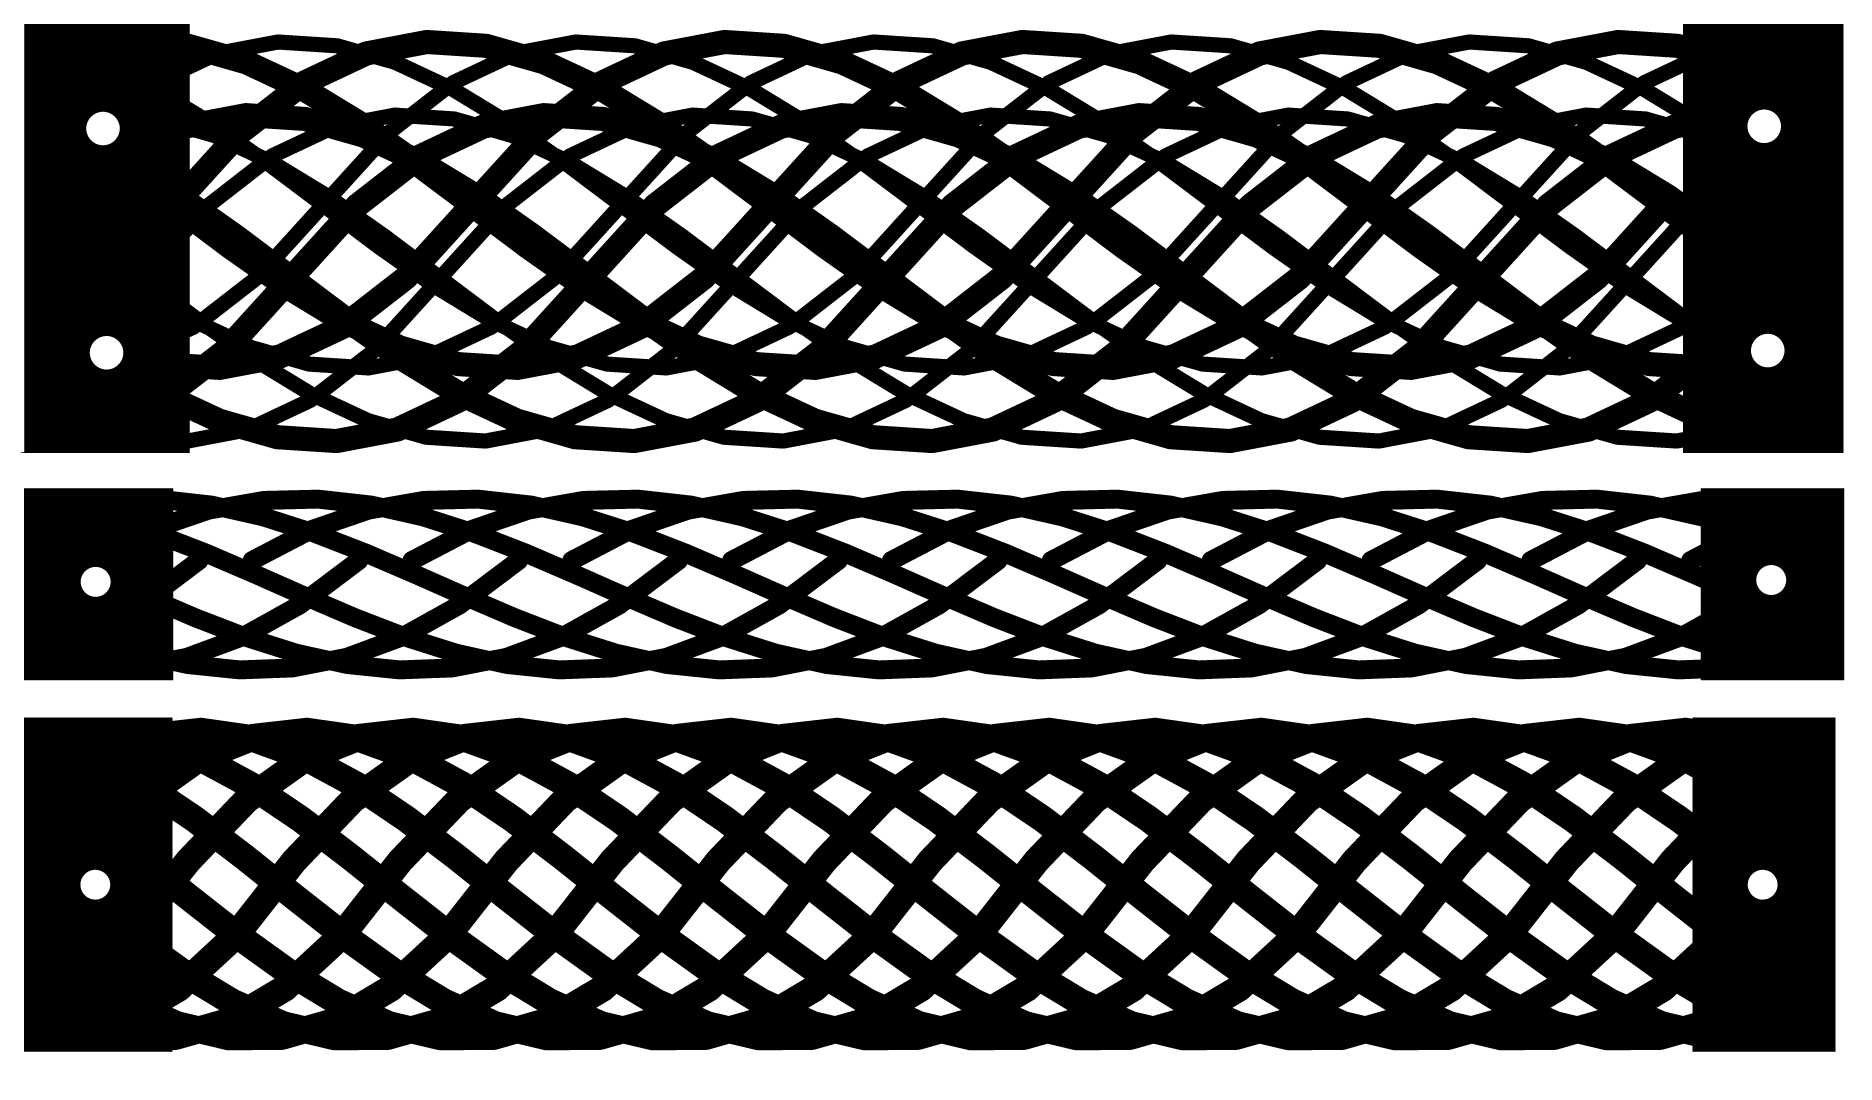
\includegraphics[width=\columnwidth]{images/weave_bracelets.png}
\caption{Alternative bracelet aesthetics}
\label{fig:weave_bracelets}
\end{figure}
\end{center}

\subsection{Emergence of Personal Value}
With Codeable Objects, Soft Objects and DressCode, it was possible for people to create objects that were beautiful. The aesthetic properties of an artifact are important indicators of success, but algorithmic craft is also capable of producing artifacts that have value beyond their physical beauty. When we asked participants to evaluate their designs, they talked about more than how the object looked. Many participants described the unique quality of their piece:

\begin{quotation}
\textit{``I think it's interesting. I'm assuming this design is unique to me unless someone else goes and makes exactly the same thing, which I highly doubt because of all the random calibration things that I ended up adding."}
\\Youth Participant C
\end{quotation}

\begin{quotation}
Youth Participant C: \textit{``You can�t find it at American eagle. I buy a lot of my bracelets there, and you can�t just go there and find this. I think it�s cool if someone were to say �Oh were did you get that from�, �You can�t find it�. (Laughs). "}
\\Interviewer:\textit{``You can say that you made it yourself, you love how it�s unique?"}
\\YouthParticipant C: \textit{``yeah"}
\end{quotation}

Some of the participants also described how their personal preferences played a strong part in the design of the piece. 

\begin{quotation}
\textit{``usually when you make something you're making it like �oh I hope society likes this� but this[making the bracelet] was about self satisfaction, so I don't have to take into consideration someone else's opinion."}
\\Youth Participant S
\end{quotation}

Comments like these demonstrate participants' awareness of the value in personal craft  practices, in contrast to commercial forms of production. The youth participants entered the workshop with no awareness of the artisanal craft, instead defining craft by its high level of accessibility. By the workshops completion however, the participants described recognized elements of craftsmanship in their own work, including uniqueness, exclusivity and personal relevancy. These qualities translated to the creator attaching a greater value to the artifact. In combination with the recognition of the craft-value of their pieces, participants also valued the artifacts because they were created withprogramming. People responded in the following ways when asked to describe their finished piece:
 
\begin{quotation}
 \textit{``II think [the programming] kind of reminded me of learning something difficult in like math, because I don't really like math, but when I figure out something, then I start doing it, and can do it and then I feel proud of myself"}
 \\Youth Participant C
\end{quotation}

 \begin{quotation}
 Interviewer:  \textit{``What stands out to you about your design?"}
 \\Youth Participant S.M.: \textit{``That I actually created it. I'm not really a programming person, doing it and typing it out."}
 \end{quotation}
 
 \begin{quotation}
Youth Participant J: \textit{``It's on computers and I'm terrible at computers and for me to actually get something like this is really big."} 
\\Interviewer:  \textit{``How do you feel about that?"}
\\Youth Participant J:  \textit{``Really proud."}	
\end{quotation}

At the end of the workshop, participants talked explicitly about the value in being exposed to programming in new ways, and their desire to continue working in computational design and digital fabrication.

 \begin{quotation}
\textit{``I don't know if this is my preferred medium, but I definitely like it.  Making other accessories. If I spent more time playing around with it, I could definitely get something good. 
I'm glad I did it, it's interesting, It's something that I don't have a lot of experience in- just branching out."}
\\Youth Participant R
\end{quotation}

\begin{quotation}
 \textit{``I thought it was a good experience, It was different and it sort of opens your mind to thinking about what else you could do with programming, fashion and stuff like that."}
 \\Youth Participant J
 \end{quotation} 
 
 \begin{quotation}
\textit{``I would love to get into more computational design, I think it's really really cool, because I'm an amateur graphic designer as well."}
\\Youth Participant ST
\end{quotation}

It is apparent that participants not only valued the artifacts they created, but also benefited from the process of producing them. The sense of pride and accomplishment in programming echoes the sentiments of the novice programers in the Soft Objects workshop. Algorithmic Craft allows people to produce unique objects that have personal and social significance beyond their appearance. Simultaneously, it introduces people to a new context for computation, while simultaneously promoting a sense of personal technological competence. The participants' desire to further engage in similar activities demonstrates the potential for the approach of algorithmic craft to promote continued engagement in programming as a creative practice.

Both computation and craft are special forms of creation. With its generative qualities, computational design can sometimes feel like alchemy. Simple shapes are transmuted to elaborate compositions, almost like magic. Craft has a different form of value, a pride in the knowledge that a piece is rare and distinct, and exists as a direct result of the hands that shaped it. Algorithmic craft provides people with the opportunity to preserve both of these forms of creation in a personal physical form. 







